% Options for packages loaded elsewhere
\PassOptionsToPackage{unicode}{hyperref}
\PassOptionsToPackage{hyphens}{url}
\PassOptionsToPackage{dvipsnames,svgnames,x11names}{xcolor}
%
\documentclass[
  letterpaper,
  DIV=11,
  numbers=noendperiod,
  oneside]{scrartcl}

\usepackage{amsmath,amssymb}
\usepackage{iftex}
\ifPDFTeX
  \usepackage[T1]{fontenc}
  \usepackage[utf8]{inputenc}
  \usepackage{textcomp} % provide euro and other symbols
\else % if luatex or xetex
  \usepackage{unicode-math}
  \defaultfontfeatures{Scale=MatchLowercase}
  \defaultfontfeatures[\rmfamily]{Ligatures=TeX,Scale=1}
\fi
\usepackage{lmodern}
\ifPDFTeX\else  
    % xetex/luatex font selection
\fi
% Use upquote if available, for straight quotes in verbatim environments
\IfFileExists{upquote.sty}{\usepackage{upquote}}{}
\IfFileExists{microtype.sty}{% use microtype if available
  \usepackage[]{microtype}
  \UseMicrotypeSet[protrusion]{basicmath} % disable protrusion for tt fonts
}{}
\makeatletter
\@ifundefined{KOMAClassName}{% if non-KOMA class
  \IfFileExists{parskip.sty}{%
    \usepackage{parskip}
  }{% else
    \setlength{\parindent}{0pt}
    \setlength{\parskip}{6pt plus 2pt minus 1pt}}
}{% if KOMA class
  \KOMAoptions{parskip=half}}
\makeatother
\usepackage{xcolor}
\usepackage[left=1in,marginparwidth=2.0666666666667in,textwidth=4.1333333333333in,marginparsep=0.3in]{geometry}
\ifLuaTeX
  \usepackage{luacolor}
  \usepackage[soul]{lua-ul}
\else
  \usepackage{soul}
  
\fi
\setlength{\emergencystretch}{3em} % prevent overfull lines
\setcounter{secnumdepth}{-\maxdimen} % remove section numbering
% Make \paragraph and \subparagraph free-standing
\makeatletter
\ifx\paragraph\undefined\else
  \let\oldparagraph\paragraph
  \renewcommand{\paragraph}{
    \@ifstar
      \xxxParagraphStar
      \xxxParagraphNoStar
  }
  \newcommand{\xxxParagraphStar}[1]{\oldparagraph*{#1}\mbox{}}
  \newcommand{\xxxParagraphNoStar}[1]{\oldparagraph{#1}\mbox{}}
\fi
\ifx\subparagraph\undefined\else
  \let\oldsubparagraph\subparagraph
  \renewcommand{\subparagraph}{
    \@ifstar
      \xxxSubParagraphStar
      \xxxSubParagraphNoStar
  }
  \newcommand{\xxxSubParagraphStar}[1]{\oldsubparagraph*{#1}\mbox{}}
  \newcommand{\xxxSubParagraphNoStar}[1]{\oldsubparagraph{#1}\mbox{}}
\fi
\makeatother

\usepackage{color}
\usepackage{fancyvrb}
\newcommand{\VerbBar}{|}
\newcommand{\VERB}{\Verb[commandchars=\\\{\}]}
\DefineVerbatimEnvironment{Highlighting}{Verbatim}{commandchars=\\\{\}}
% Add ',fontsize=\small' for more characters per line
\usepackage{framed}
\definecolor{shadecolor}{RGB}{241,243,245}
\newenvironment{Shaded}{\begin{snugshade}}{\end{snugshade}}
\newcommand{\AlertTok}[1]{\textcolor[rgb]{0.68,0.00,0.00}{#1}}
\newcommand{\AnnotationTok}[1]{\textcolor[rgb]{0.37,0.37,0.37}{#1}}
\newcommand{\AttributeTok}[1]{\textcolor[rgb]{0.40,0.45,0.13}{#1}}
\newcommand{\BaseNTok}[1]{\textcolor[rgb]{0.68,0.00,0.00}{#1}}
\newcommand{\BuiltInTok}[1]{\textcolor[rgb]{0.00,0.23,0.31}{#1}}
\newcommand{\CharTok}[1]{\textcolor[rgb]{0.13,0.47,0.30}{#1}}
\newcommand{\CommentTok}[1]{\textcolor[rgb]{0.37,0.37,0.37}{#1}}
\newcommand{\CommentVarTok}[1]{\textcolor[rgb]{0.37,0.37,0.37}{\textit{#1}}}
\newcommand{\ConstantTok}[1]{\textcolor[rgb]{0.56,0.35,0.01}{#1}}
\newcommand{\ControlFlowTok}[1]{\textcolor[rgb]{0.00,0.23,0.31}{\textbf{#1}}}
\newcommand{\DataTypeTok}[1]{\textcolor[rgb]{0.68,0.00,0.00}{#1}}
\newcommand{\DecValTok}[1]{\textcolor[rgb]{0.68,0.00,0.00}{#1}}
\newcommand{\DocumentationTok}[1]{\textcolor[rgb]{0.37,0.37,0.37}{\textit{#1}}}
\newcommand{\ErrorTok}[1]{\textcolor[rgb]{0.68,0.00,0.00}{#1}}
\newcommand{\ExtensionTok}[1]{\textcolor[rgb]{0.00,0.23,0.31}{#1}}
\newcommand{\FloatTok}[1]{\textcolor[rgb]{0.68,0.00,0.00}{#1}}
\newcommand{\FunctionTok}[1]{\textcolor[rgb]{0.28,0.35,0.67}{#1}}
\newcommand{\ImportTok}[1]{\textcolor[rgb]{0.00,0.46,0.62}{#1}}
\newcommand{\InformationTok}[1]{\textcolor[rgb]{0.37,0.37,0.37}{#1}}
\newcommand{\KeywordTok}[1]{\textcolor[rgb]{0.00,0.23,0.31}{\textbf{#1}}}
\newcommand{\NormalTok}[1]{\textcolor[rgb]{0.00,0.23,0.31}{#1}}
\newcommand{\OperatorTok}[1]{\textcolor[rgb]{0.37,0.37,0.37}{#1}}
\newcommand{\OtherTok}[1]{\textcolor[rgb]{0.00,0.23,0.31}{#1}}
\newcommand{\PreprocessorTok}[1]{\textcolor[rgb]{0.68,0.00,0.00}{#1}}
\newcommand{\RegionMarkerTok}[1]{\textcolor[rgb]{0.00,0.23,0.31}{#1}}
\newcommand{\SpecialCharTok}[1]{\textcolor[rgb]{0.37,0.37,0.37}{#1}}
\newcommand{\SpecialStringTok}[1]{\textcolor[rgb]{0.13,0.47,0.30}{#1}}
\newcommand{\StringTok}[1]{\textcolor[rgb]{0.13,0.47,0.30}{#1}}
\newcommand{\VariableTok}[1]{\textcolor[rgb]{0.07,0.07,0.07}{#1}}
\newcommand{\VerbatimStringTok}[1]{\textcolor[rgb]{0.13,0.47,0.30}{#1}}
\newcommand{\WarningTok}[1]{\textcolor[rgb]{0.37,0.37,0.37}{\textit{#1}}}

\providecommand{\tightlist}{%
  \setlength{\itemsep}{0pt}\setlength{\parskip}{0pt}}\usepackage{longtable,booktabs,array}
\usepackage{calc} % for calculating minipage widths
% Correct order of tables after \paragraph or \subparagraph
\usepackage{etoolbox}
\makeatletter
\patchcmd\longtable{\par}{\if@noskipsec\mbox{}\fi\par}{}{}
\makeatother
% Allow footnotes in longtable head/foot
\IfFileExists{footnotehyper.sty}{\usepackage{footnotehyper}}{\usepackage{footnote}}
\makesavenoteenv{longtable}
\usepackage{graphicx}
\makeatletter
\newsavebox\pandoc@box
\newcommand*\pandocbounded[1]{% scales image to fit in text height/width
  \sbox\pandoc@box{#1}%
  \Gscale@div\@tempa{\textheight}{\dimexpr\ht\pandoc@box+\dp\pandoc@box\relax}%
  \Gscale@div\@tempb{\linewidth}{\wd\pandoc@box}%
  \ifdim\@tempb\p@<\@tempa\p@\let\@tempa\@tempb\fi% select the smaller of both
  \ifdim\@tempa\p@<\p@\scalebox{\@tempa}{\usebox\pandoc@box}%
  \else\usebox{\pandoc@box}%
  \fi%
}
% Set default figure placement to htbp
\def\fps@figure{htbp}
\makeatother

\KOMAoption{captions}{tableheading}
\makeatletter
\@ifpackageloaded{float}{}{\usepackage{float}}
\floatstyle{plain}
\@ifundefined{c@chapter}{\newfloat{algo}{h}{loalgo}}{\newfloat{algo}{h}{loalgo}[chapter]}
\floatname{algo}{Algorithm}
\newcommand*\listofalgos{\listof{algo}{List of Algorithms}}
\makeatother
\makeatletter
\@ifpackageloaded{tcolorbox}{}{\usepackage[skins,breakable]{tcolorbox}}
\@ifpackageloaded{fontawesome5}{}{\usepackage{fontawesome5}}
\definecolor{quarto-callout-color}{HTML}{909090}
\definecolor{quarto-callout-note-color}{HTML}{0758E5}
\definecolor{quarto-callout-important-color}{HTML}{CC1914}
\definecolor{quarto-callout-warning-color}{HTML}{EB9113}
\definecolor{quarto-callout-tip-color}{HTML}{00A047}
\definecolor{quarto-callout-caution-color}{HTML}{FC5300}
\definecolor{quarto-callout-color-frame}{HTML}{acacac}
\definecolor{quarto-callout-note-color-frame}{HTML}{4582ec}
\definecolor{quarto-callout-important-color-frame}{HTML}{d9534f}
\definecolor{quarto-callout-warning-color-frame}{HTML}{f0ad4e}
\definecolor{quarto-callout-tip-color-frame}{HTML}{02b875}
\definecolor{quarto-callout-caution-color-frame}{HTML}{fd7e14}
\makeatother
\makeatletter
\@ifpackageloaded{caption}{}{\usepackage{caption}}
\AtBeginDocument{%
\ifdefined\contentsname
  \renewcommand*\contentsname{Table of contents}
\else
  \newcommand\contentsname{Table of contents}
\fi
\ifdefined\listfigurename
  \renewcommand*\listfigurename{List of Figures}
\else
  \newcommand\listfigurename{List of Figures}
\fi
\ifdefined\listtablename
  \renewcommand*\listtablename{List of Tables}
\else
  \newcommand\listtablename{List of Tables}
\fi
\ifdefined\figurename
  \renewcommand*\figurename{Figure}
\else
  \newcommand\figurename{Figure}
\fi
\ifdefined\tablename
  \renewcommand*\tablename{Table}
\else
  \newcommand\tablename{Table}
\fi
}
\@ifpackageloaded{float}{}{\usepackage{float}}
\floatstyle{ruled}
\@ifundefined{c@chapter}{\newfloat{codelisting}{h}{lop}}{\newfloat{codelisting}{h}{lop}[chapter]}
\floatname{codelisting}{Listing}
\newcommand*\listoflistings{\listof{codelisting}{List of Listings}}
\usepackage{amsthm}
\theoremstyle{definition}
\newtheorem{example}{Example}[section]
\theoremstyle{remark}
\AtBeginDocument{\renewcommand*{\proofname}{Proof}}
\newtheorem*{remark}{Remark}
\newtheorem*{solution}{Solution}
\newtheorem{refremark}{Remark}[section]
\newtheorem{refsolution}{Solution}[section]
\makeatother
\makeatletter
\makeatother
\makeatletter
\@ifpackageloaded{caption}{}{\usepackage{caption}}
\@ifpackageloaded{subcaption}{}{\usepackage{subcaption}}
\makeatother
\makeatletter
\@ifpackageloaded{sidenotes}{}{\usepackage{sidenotes}}
\@ifpackageloaded{marginnote}{}{\usepackage{marginnote}}
\makeatother

\usepackage{bookmark}

\IfFileExists{xurl.sty}{\usepackage{xurl}}{} % add URL line breaks if available
\urlstyle{same} % disable monospaced font for URLs
\hypersetup{
  pdftitle={The K-Armed Bandit Problem},
  pdfauthor={Oren Bochman},
  colorlinks=true,
  linkcolor={blue},
  filecolor={Maroon},
  citecolor={Blue},
  urlcolor={Blue},
  pdfcreator={LaTeX via pandoc}}


\title{The K-Armed Bandit Problem}
\usepackage{etoolbox}
\makeatletter
\providecommand{\subtitle}[1]{% add subtitle to \maketitle
  \apptocmd{\@title}{\par {\large #1 \par}}{}{}
}
\makeatother
\subtitle{RL Fundamentals}
\author{Oren Bochman}
\date{2022-05-02}

\begin{document}
\maketitle

\numberwithin{algorithm}{chapter}
\algrenewcommand{\algorithmiccomment}[1]{\hskip3em$\rightarrow$ #1}


\begin{figure}[H]

{\centering \pandocbounded{\includegraphics[keepaspectratio]{img/logo.png}}

}

\caption{RL logo}

\end{figure}%%
\begin{figure}[H]

{\centering \pandocbounded{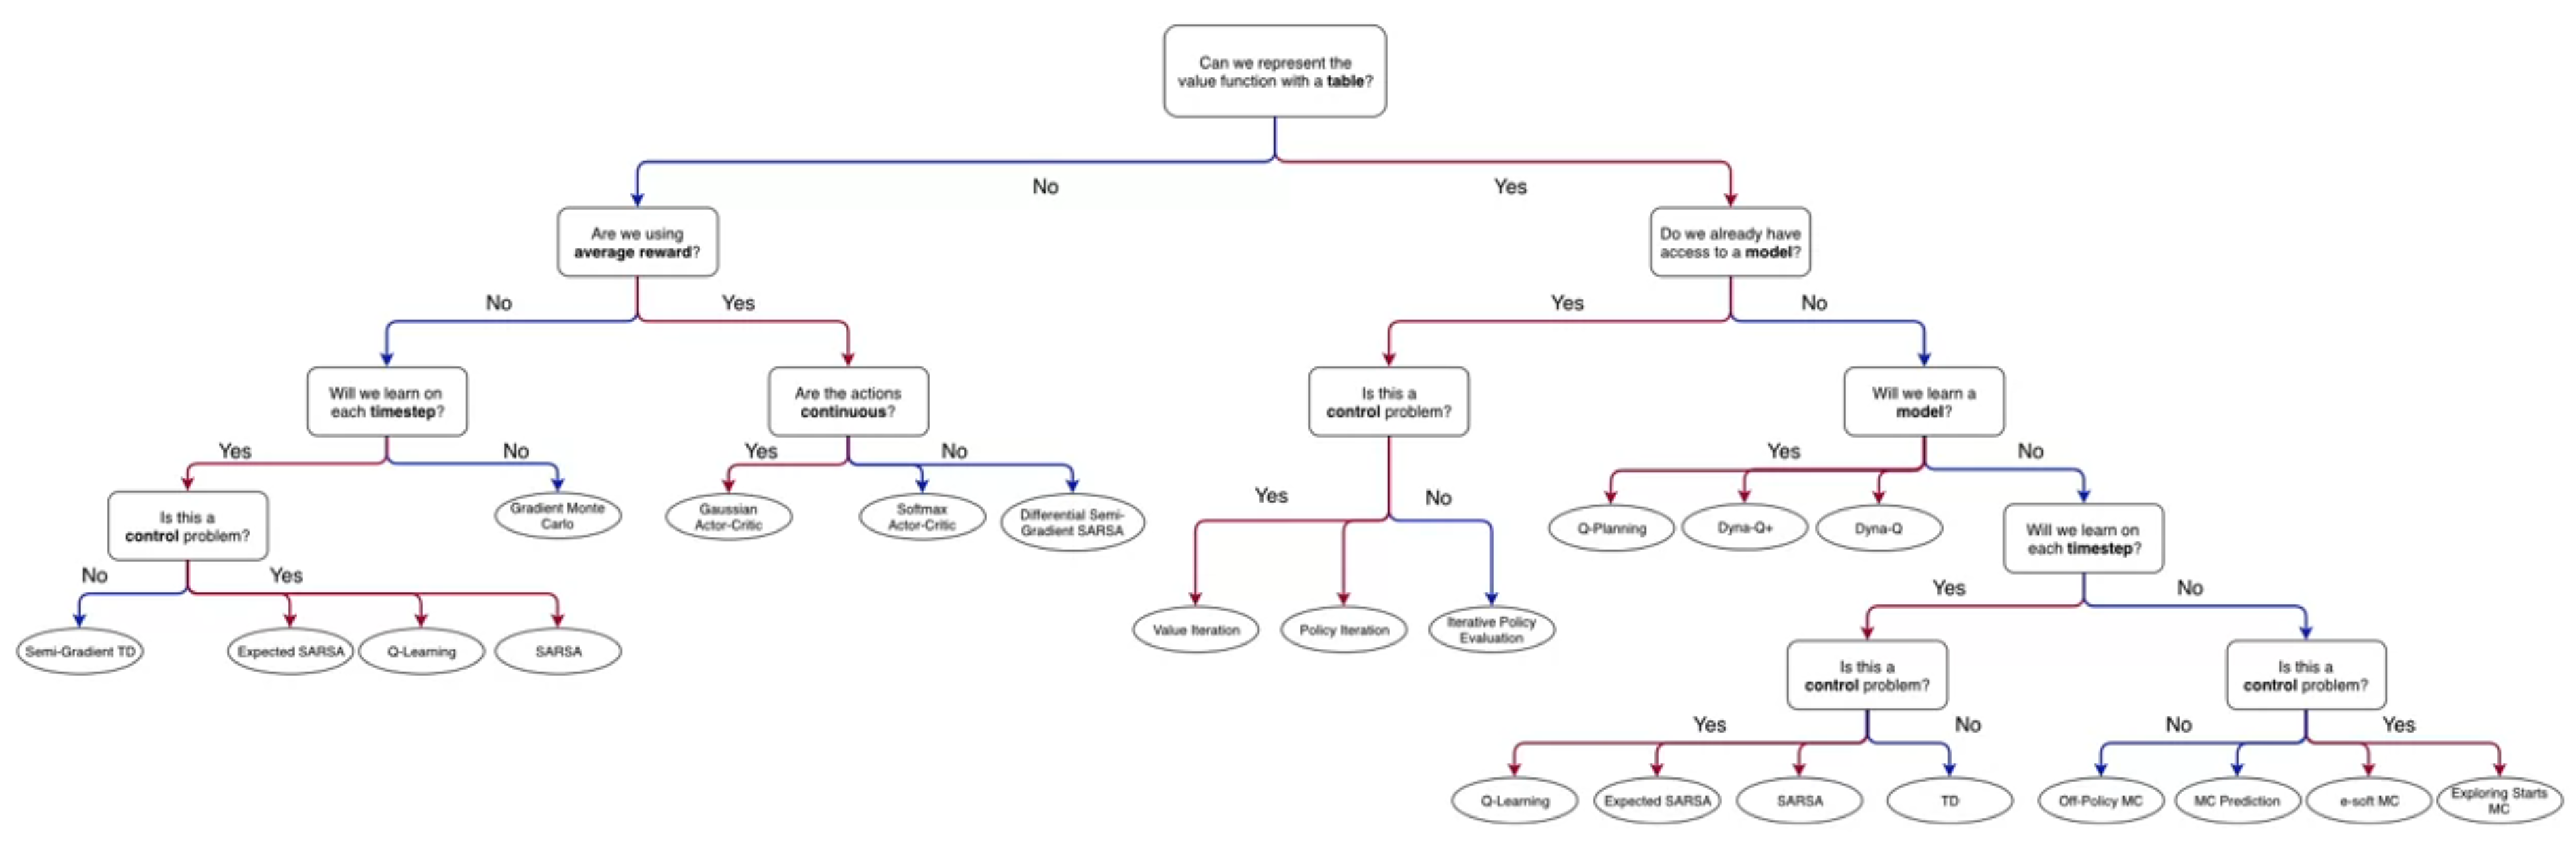
\includegraphics[keepaspectratio]{img/alg_selector.png}}

}

\caption{RL algorithms}

\end{figure}%

\section{Lesson 1: The K-Armed Bandit}\label{sec-lesson-k-armed-bandit}

\begin{tcolorbox}[enhanced jigsaw, left=2mm, leftrule=.75mm, bottomtitle=1mm, toptitle=1mm, title=\textcolor{quarto-callout-tip-color}{\faLightbulb}\hspace{0.5em}{Read}, breakable, toprule=.15mm, colbacktitle=quarto-callout-tip-color!10!white, coltitle=black, colback=white, opacityback=0, rightrule=.15mm, bottomrule=.15mm, colframe=quarto-callout-tip-color-frame, titlerule=0mm, opacitybacktitle=0.6, arc=.35mm]

\begin{itemize}
\tightlist
\item[$\boxtimes$]
  \href{http://incompleteideas.net/book/RLbook2020.pdf\#page=47}{@sutton2018reinforcement§2.1-7,
  pp.~25-36}
\item[$\boxtimes$]
  \href{http://incompleteideas.net/book/RLbook2020.pdf\#page=47}{@sutton2018reinforcement§2.8,
  pp.~42-43}
\end{itemize}

\end{tcolorbox}

\begin{tcolorbox}[enhanced jigsaw, left=2mm, leftrule=.75mm, bottomtitle=1mm, toptitle=1mm, title=\textcolor{quarto-callout-note-color}{\faInfo}\hspace{0.5em}{Goals}, breakable, toprule=.15mm, colbacktitle=quarto-callout-note-color!10!white, coltitle=black, colback=white, opacityback=0, rightrule=.15mm, bottomrule=.15mm, colframe=quarto-callout-note-color-frame, titlerule=0mm, opacitybacktitle=0.6, arc=.35mm]

\begin{itemize}
\tightlist
\item[$\boxtimes$]
  Understand the temporal nature of the bandit problem
  \hyperref[sec-k-armed-bandit]{\#}
\item[$\boxtimes$]
  Define k-armed bandit problem \hyperref[l1g2]{\#}
\item[$\boxtimes$]
  Define action-values and the greedy action selection method
  \hyperref[sec-l1g3]{\#}
\item[$\boxtimes$]
  Define reward, time steps, and value functions \hyperref[l1g4]{\#}
\end{itemize}

\end{tcolorbox}

\begin{quote}
In reinforcement learning, the agent generates its own training data by
interacting with the world. The agent must learn the consequences of his
own actions through trial and error, rather than being told the correct
action -- {[}@white2020fundamental{]}
\end{quote}

\subsection{K-armed bandits 🐙}\label{sec-k-armed-bandit}

In the \textbf{k-armed bandit} problem there is an \textbf{agent} who is
assigned a \textbf{state} \(s\) by the environment and must learn which
action \(a\) from the possible set of \textbf{actions} \(A\) leads to
the goal state through a signal based on the greatest \textbf{expected
reward}.

One way this can be achieved is using a Bayesian updating scheme
starting from a uniform prior.

\subsection{Temporal nature of the bandit problem}\label{sec-l1g1}

The \textbf{bandit problem} cam be static problem with a fixed reward
distribution. However, more generally it is a \textbf{temporal} problem
when the rewards distribution changes over time and agent must learn to
adapt to these changes.

\begin{tcolorbox}[enhanced jigsaw, left=2mm, leftrule=.75mm, bottomtitle=1mm, toptitle=1mm, title=\textcolor{quarto-callout-note-color}{\faInfo}\hspace{0.5em}{Difference between bandits and RL}, breakable, toprule=.15mm, colbacktitle=quarto-callout-note-color!10!white, coltitle=black, colback=white, opacityback=0, rightrule=.15mm, bottomrule=.15mm, colframe=quarto-callout-note-color-frame, titlerule=0mm, opacitybacktitle=0.6, arc=.35mm]

In the typical \textbf{bandit setting} there is only one state. So after
we pull the arm nothing in the problem changes.

Bandits problems where agents can discriminate between states are called
\emph{contextual bandits.}

However, bandits embody one of the main themes of RL - that of
estimating an expected reward for different actions.

In the more general \textbf{RL setting} we will be interested in more
general problems where actions will lead the agent to new states and the
goal is some specific state we need to reach.

\end{tcolorbox}

\begin{figure}[H]

{\centering \pandocbounded{\includegraphics[keepaspectratio]{img/multi_armed_bandit.webm}}

}

\caption{bandit}

\end{figure}%

\begin{example}[Using Multi-armed bandit to randomize a medical
trial]\protect\hypertarget{exm-clinical-trials}{}\label{exm-clinical-trials}

~

\begin{itemize}
\tightlist
\item
  agent is the doctor
\item
  actions \{blue, yellow, red\} treatment
\item
  k = 3
\item
  the rewards are the health of the patients' blood pressure.
\item
  a random trial in which a doctor need to pick one of three treatments.
\item
  q(a) is the mean of the blood pressure for the patient.
\end{itemize}

\end{example}

\begin{figure}[H]

{\centering \pandocbounded{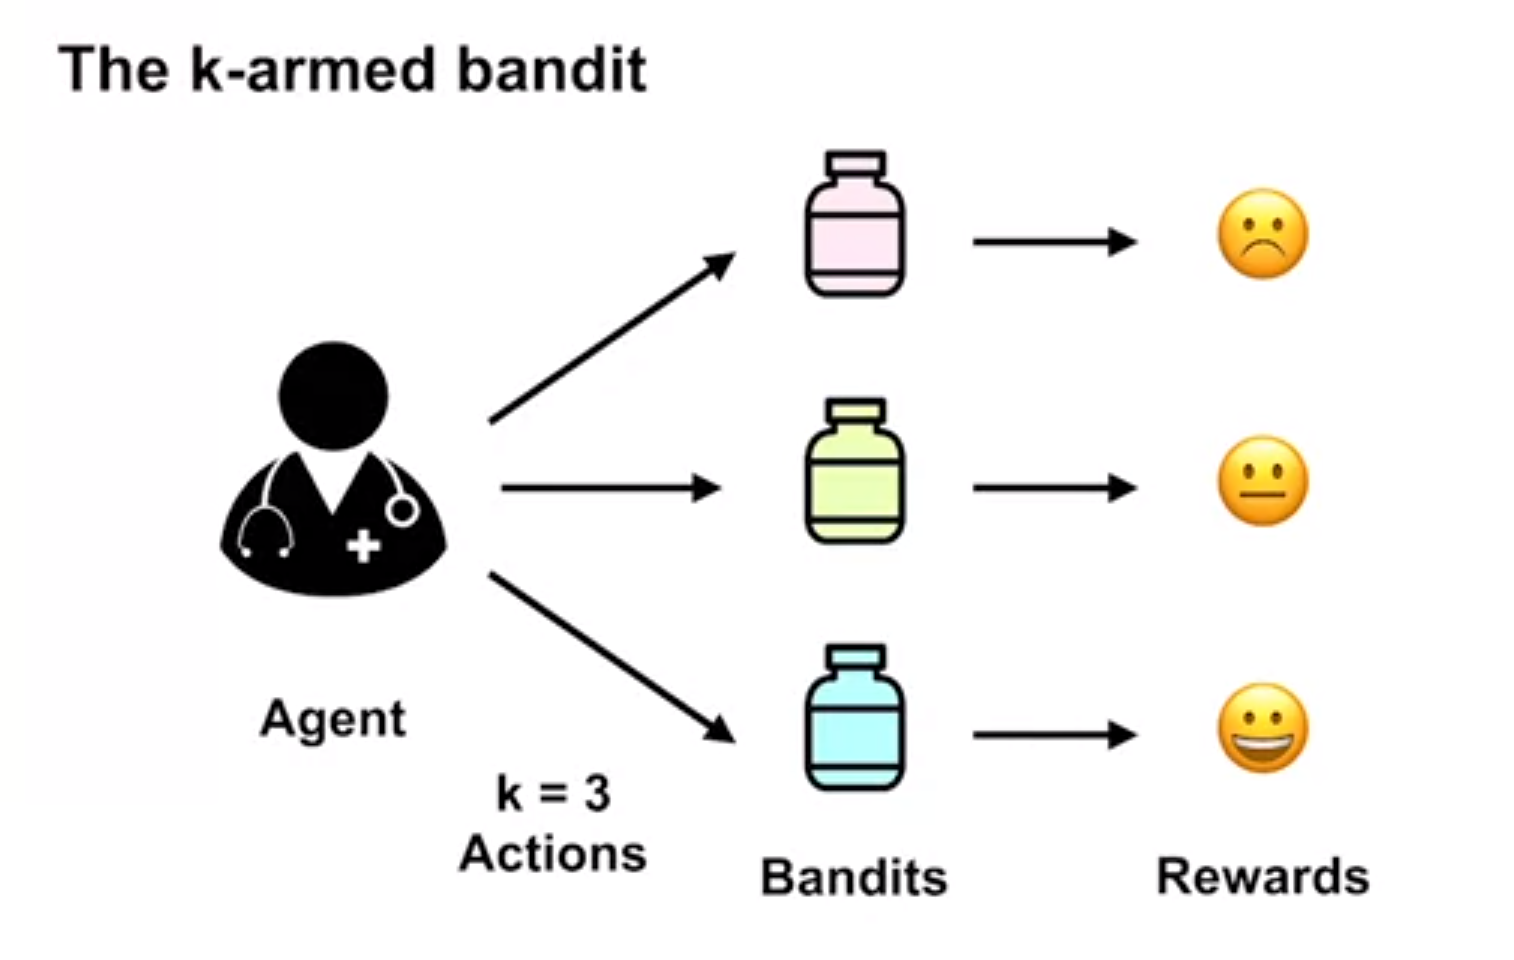
\includegraphics[keepaspectratio]{img/rl-clinical-trial.png}}

}

\caption{clinical trial}

\end{figure}%

\paragraph{Action Values and Greedy Action Selection}\label{sec-l1g3}

The \textbf{value} of an action is its \textbf{expected reward} which
can be expressed mathematically as:

\begin{equation}\phantomsection\label{eq-action-value}{
\begin{align}
q_{\star}(a) & \doteq \mathbb{E}[R_t  \vert  A_t=a] \space \forall a \in \{a_1 ... a_k\} \newline 
             & = \sum_r p(r|a)r \qquad \text{(action value)}
\end{align}
}\end{equation}

where:

\begin{itemize}
\tightlist
\item
  \(\doteq\) means definition
\item
  \(\mathbb{E}[r \vert a]\) means expectation of a reward given some
  action a Since agents want to maximize rewards, recalling the
  definition of expectations we can write this as:
\end{itemize}

The goal of the agent is to maximize the expected reward which we can
express mathematically as:

\begin{equation}\phantomsection\label{eq-greedification}{
 \arg\max_a q(a)=\sum_r p(r \vert a) \times r \qquad \text{(Greedification)}
}\end{equation}

where:

\begin{itemize}
\tightlist
\item
  \(\arg \max_a\) means the argument \(a\) maximizes - so the agent is
  looking for the action that maximizes the expected reward and the
  outcome is an action.
\end{itemize}

\paragraph{Reward, Return, and Value Functions}\label{l1g4}

The \textbf{reward} \(r\) is the immediate feedback from the environment
after the agent takes an action.

The \textbf{return} \(G_t\) is the total discounted reward from
time-step \(t\).

The \textbf{value function} \(v(s)\) of an MRP is the expected return
starting from state \(s\).

\begin{figure}[H]

{\centering \pandocbounded{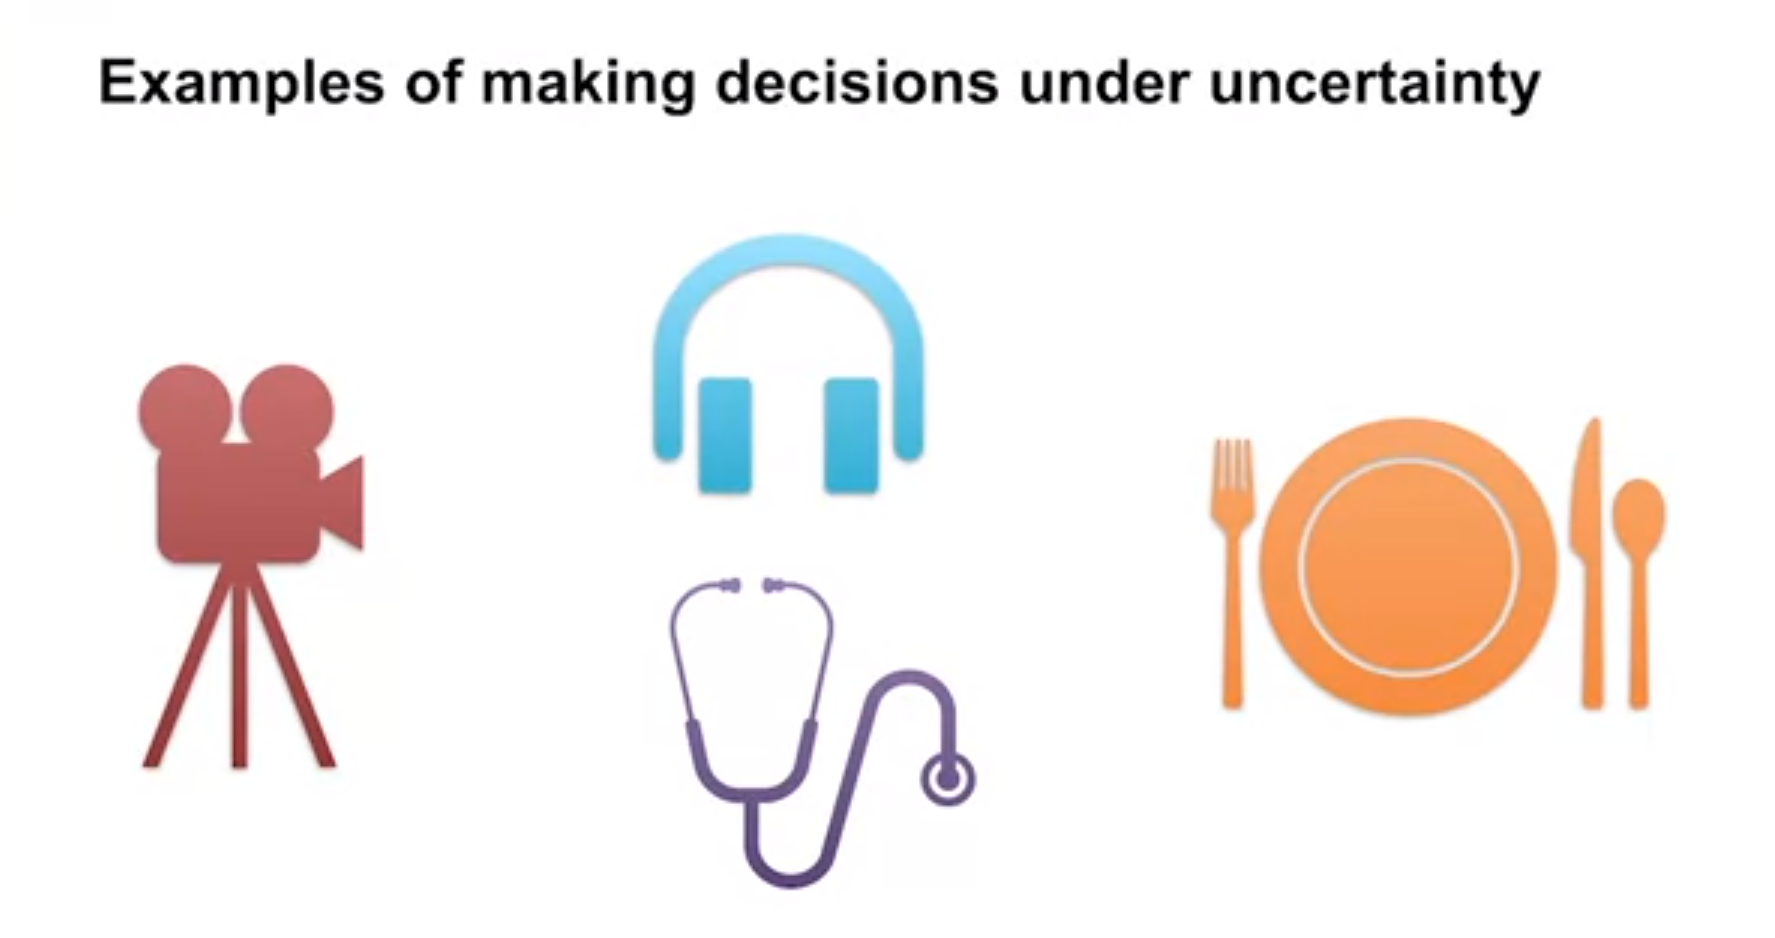
\includegraphics[keepaspectratio]{img/rl-descion-problems.png}}

}

\caption{decisions}

\end{figure}%

example of decisions under uncertainty:

\begin{itemize}
\tightlist
\item
  movie recommendation.
\item
  clinical trials.
\item
  music recommendation.
\item
  food ordering at a restaurant.
\end{itemize}

\begin{figure}[H]

{\centering \pandocbounded{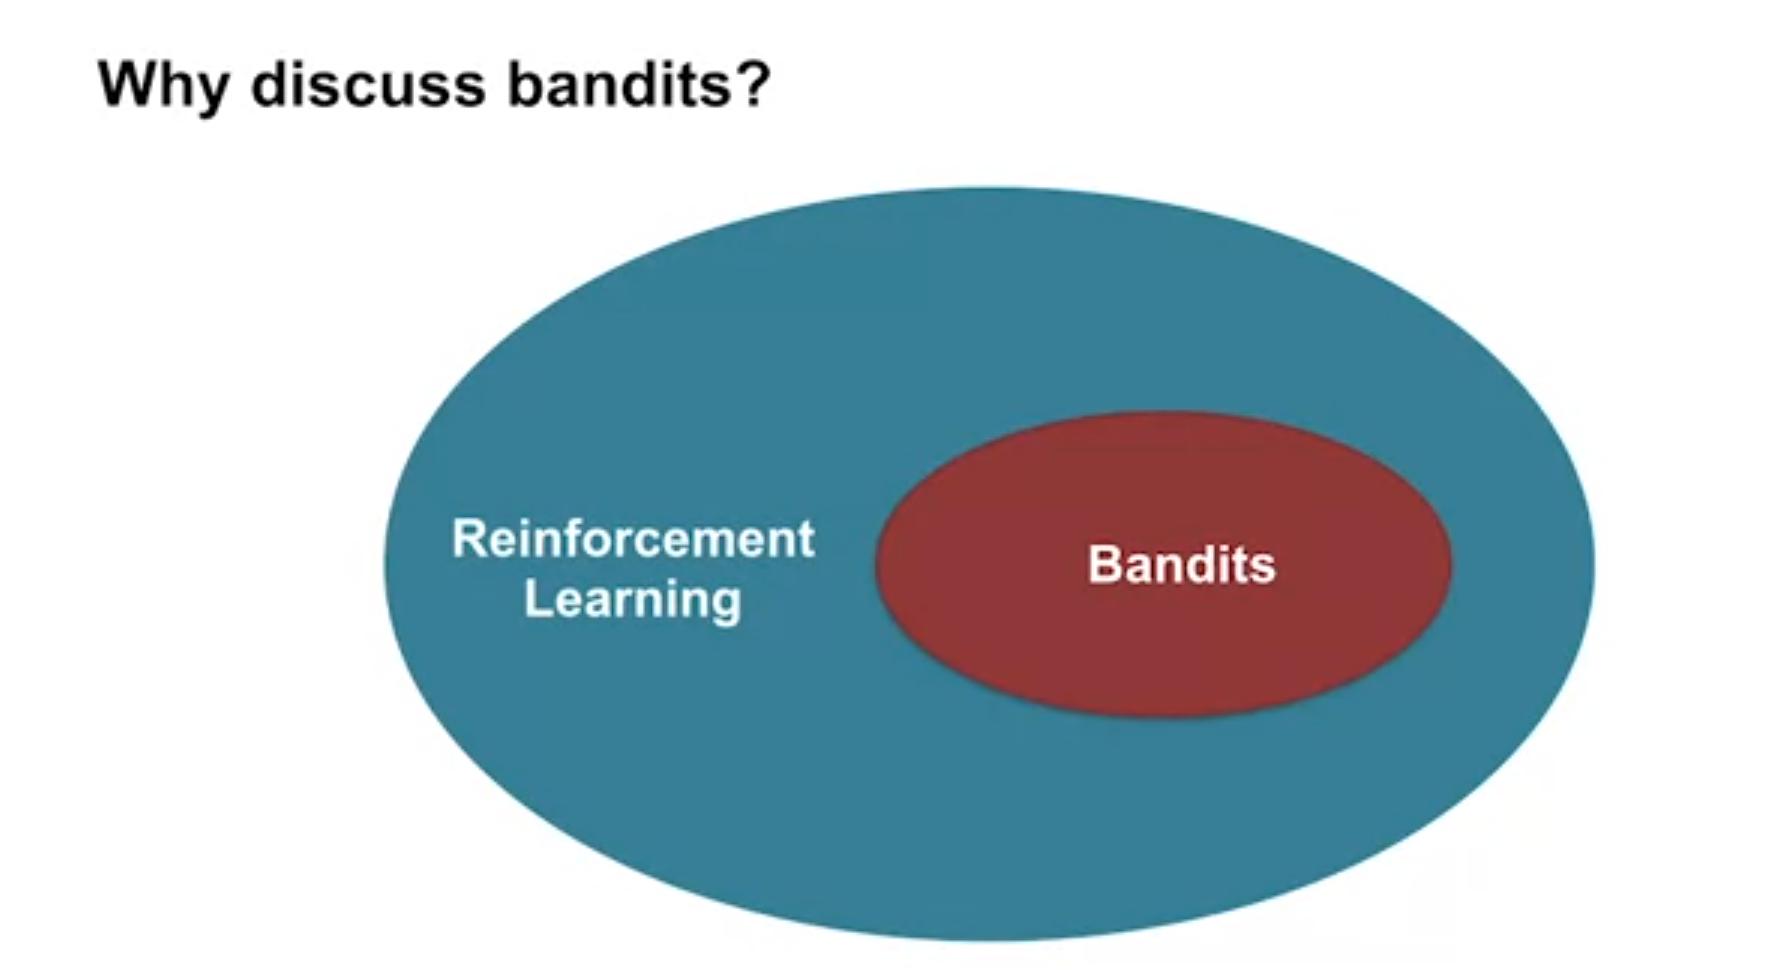
\includegraphics[keepaspectratio]{img/rl-why-bandits.png}}

}

\caption{why discuss bandits}

\end{figure}%

It best to consider issues and algorithms design choices in the simplest
setting first. The bandit problem is the simplest setting for RL. More
advanced algorithms will incorporate parts we use to solve this simple
settings.

\begin{itemize}
\tightlist
\item
  maximizing rewards.
\item
  balancing exploration and exploitation.
\item
  estimating expected rewards for different actions.
\end{itemize}

are all problems we will encounter in both the bandit and the more
general RL setting.

\section{Lesson 2: What to learn: understanding Action
Values}\label{sec-lesson-action-values}

\begin{tcolorbox}[enhanced jigsaw, left=2mm, leftrule=.75mm, bottomtitle=1mm, toptitle=1mm, title=\textcolor{quarto-callout-note-color}{\faInfo}\hspace{0.5em}{Goals}, breakable, toprule=.15mm, colbacktitle=quarto-callout-note-color!10!white, coltitle=black, colback=white, opacityback=0, rightrule=.15mm, bottomrule=.15mm, colframe=quarto-callout-note-color-frame, titlerule=0mm, opacitybacktitle=0.6, arc=.35mm]

\begin{enumerate}
\def\labelenumi{\arabic{enumi}.}
\tightlist
\item
  ☒ Define action-value estimation methods. \hyperref[L2G1]{\#}
\item
  ☒ Define exploration and exploitation \hyperref[L2G2]{\#}
\item
  ☒ Select actions greedily using an action-value function
  \hyperref[L2G3]{\#}
\item
  ☒ Define online learning \hyperref[L2G4]{\#}
\item
  ☒ Understand a simple online sample-average action-value estimation
  method \hyperref[L2G5]{\#}
\item
  ☒ Define the general online update equation \hyperref[L2G6]{\#}
\end{enumerate}

\end{tcolorbox}

\subsubsection{What are action-value estimation methods?}\label{L2G1}

\begin{figure}[H]

{\centering \pandocbounded{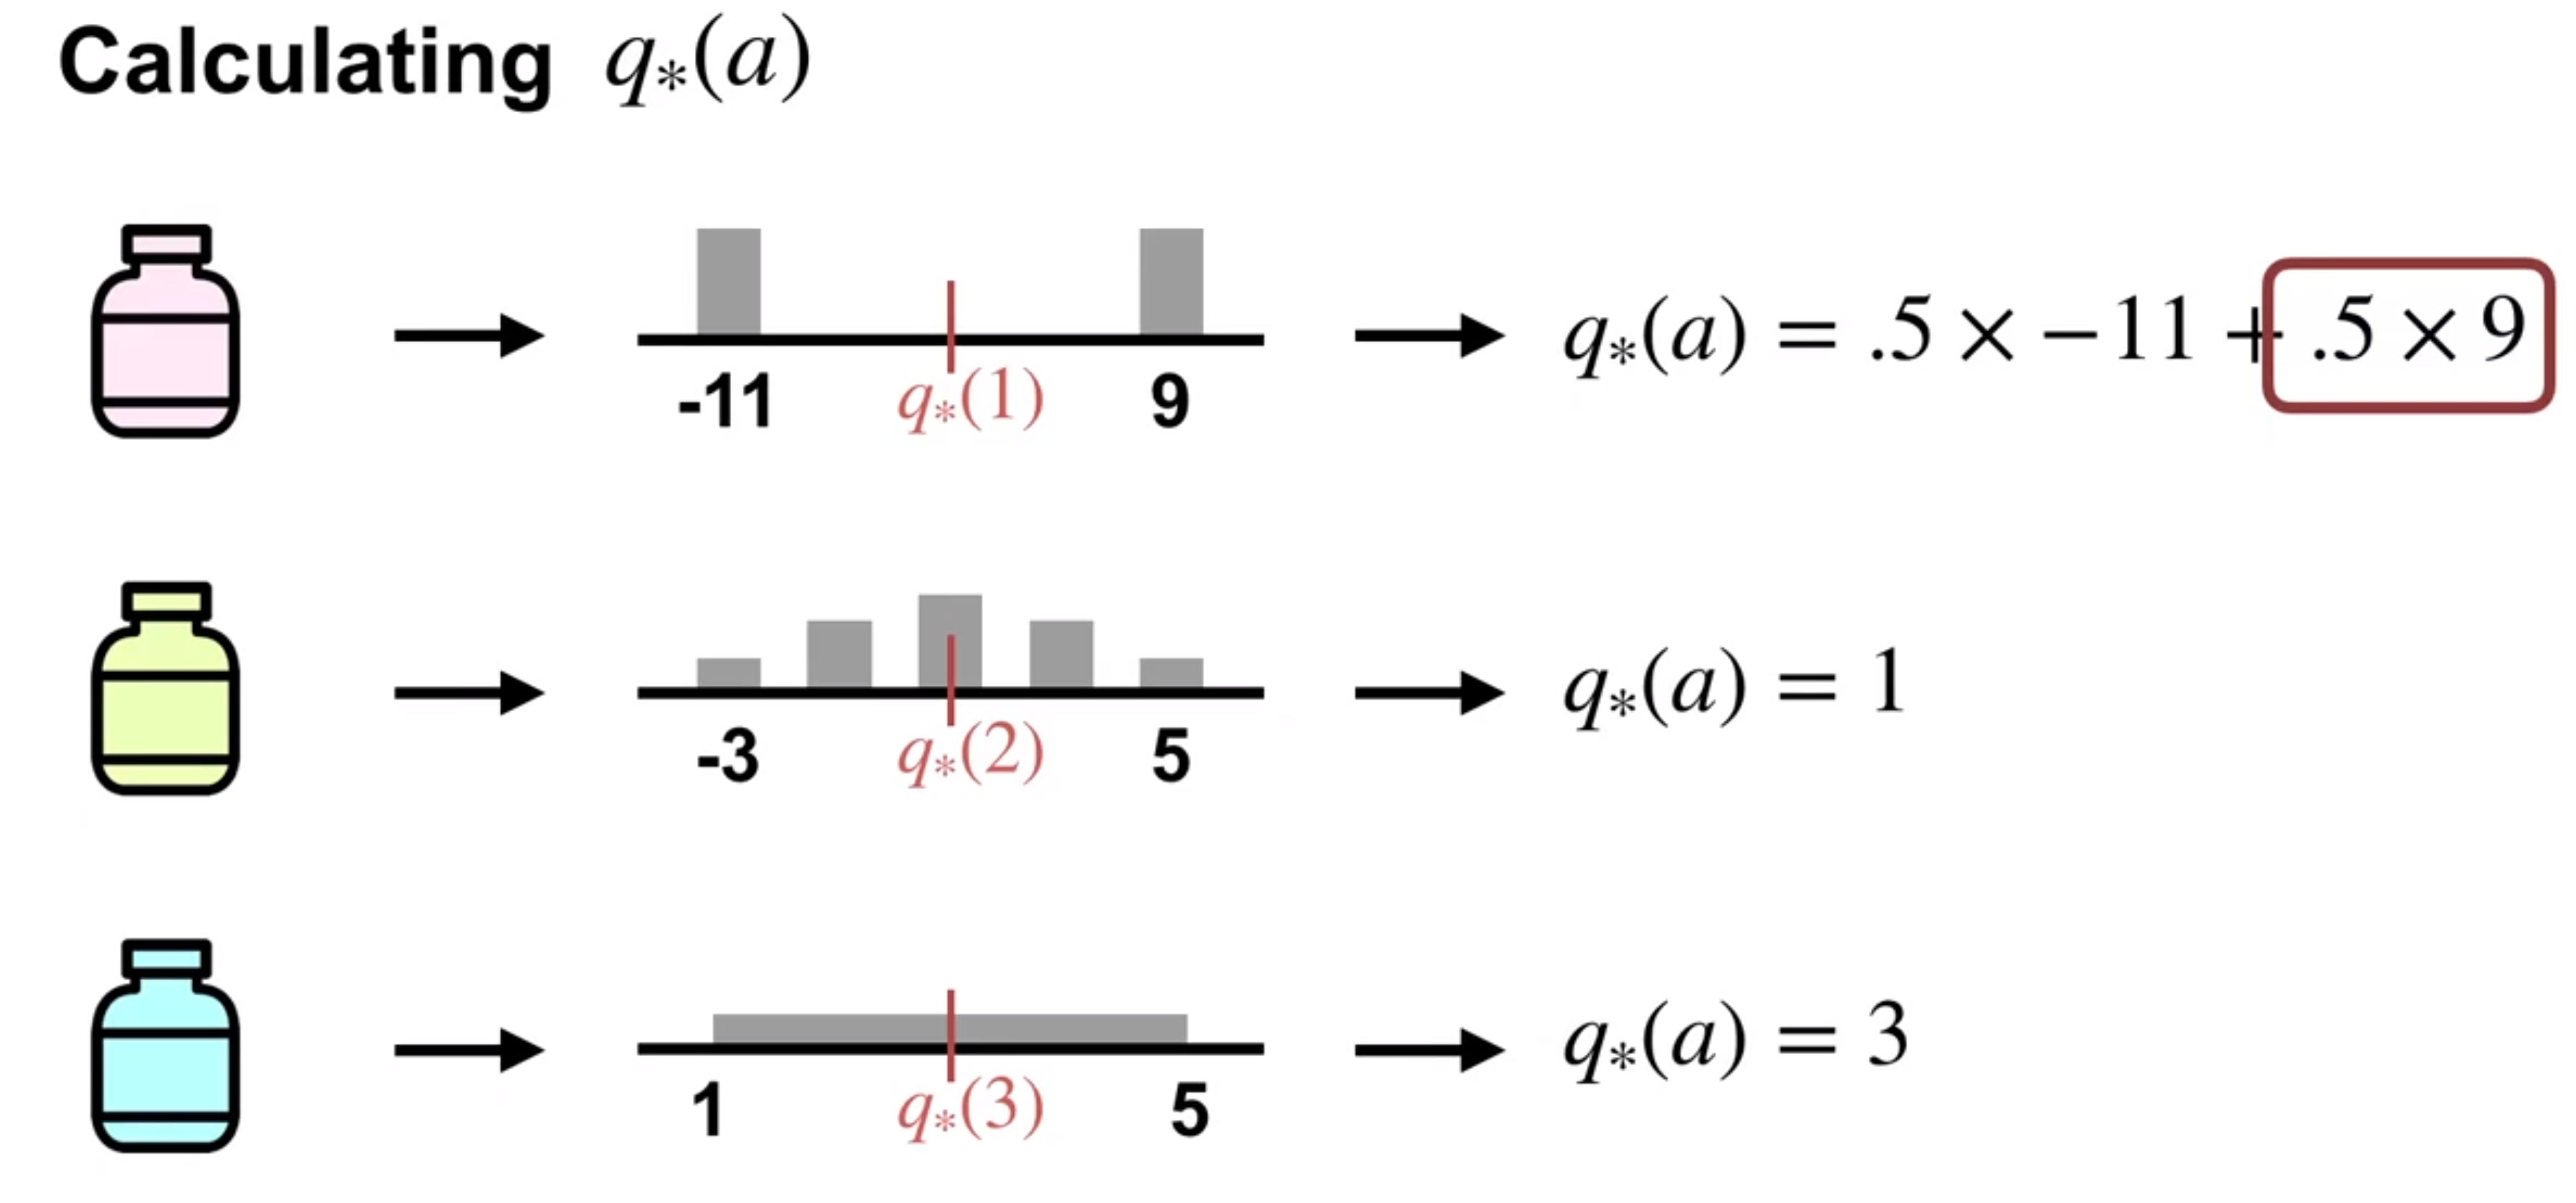
\includegraphics[keepaspectratio]{img/rl-clinical-trial-q(a).png}}

}

\caption{estimating action values}

\end{figure}%

In Tabular RL settings The action value function \(q\) is nothing more
than a table with one \{state, action\} pair per row and its value. More
generally, like when we will consider function approximation in course
3, it is a mapping from \{state, action\} pair to a expected reward.

\begin{longtable}[]{@{}lll@{}}
\toprule\noalign{}
State s & Action a & Action value q(s,a) \\
\midrule\noalign{}
\endhead
\bottomrule\noalign{}
\endlastfoot
0 & red treatment & 0.25 \\
0 & yellow treatment & 0.75 \\
0 & blue treatment & 0.5 \\
\end{longtable}

The higher the action value \(q(a)\) of an action \textbf{a}, the more
likely it is to lead us to a better state which is closer to the
objective. We can choose for each state the best or one of the best
choices giving us a \textbf{plan} for navigating the state space to the
goal state.

\begin{equation}\phantomsection\label{eq-sample-average}{
Q_t(a) \doteq \frac{\text{sum of rewards for action a taken time } t}{\text{number of times action a was taken prior to } t} = \frac{\sum_{i=1}^{t-1} R_i}{t-1} \qquad
}\end{equation}

The main idea of RL is that we can propagate values from an one adjacent
state to another. We can start with the uniform stochastic policy and
use it to estimate/learn the action values. Action values will decrease
for actions leads to a dead end. And it will increase in the direction
of the goal but only once the influence of the goal has propagated. A
continuing theme in RL is trying to increase the efficiency for
propagation of rewards across the action values.

Knowing the minimum number of action needed to reach a goal can be an
approximate indicator of the action value.

A second idea is that once we have let the influence of dead end and the
goals spread enough we may have enough information to improve the
initial action value to a point where each action is the one of the best
choices. \hl{We call picking the one of the best action greedy selection
and it leads to a deterministic policy.} This is the optimal policy, it
might not be unique since some actions might be tied in terms of their
rewards. However for all of these we cannot do any better.

\subsubsection{Exploration and Exploitation definition and
dilemma}\label{L2G2}

In the bandit setting we can define:

\begin{description}
\item[Exploration]
Testing any action that might be better than our best.
\item[Exploitation]
Using the best action.
\end{description}

Should the doctor explore new treatments that might harm his patients or
exploit the current treatment. In real life bacteria gain immunity to
antibiotics so there is merit to exploring new treatments. However, a
new treatment can be harmful to some patients. Ideally we want to enjoy
the benefits of the best treatment but to be open to new and better
alternatives but we can only do one at a time.

{Since exploitation is by definition mutually exclusive with exploration
we must choose one and give up the benefits of the other. This is the
\textbf{dilemma of Exploration and Exploitation}.} How an agent resolves
this dilemma in practice depends on the agent's preferences and the type
of state space it inhabits, if it has just started or encounters a
\textbf{changing landscape,} it should make an effort to explore, on the
other hand if it has explored enough to be certain of a global maximum
it would prefer to exploit.

\subsubsection{Defining Online learning ?}\label{L2G4}

\begin{description}
\item[Online learning]
learning by updating the agent's value function or the action value
function step by step as an agent transverses the states seeking the
goal. Online learning is important to handle MDP which can change.
\end{description}

One simple way an agent can use online learning is to try actions by
random and keep track of the subsequent states. Eventually we should
reach the goal state. If we repeat this many times we can estimate the
expected rewards for each action.

\subsubsection{Sample Average Method for estimating Action Values
Incrementally}\label{L2G5}

Action values help us make decision. Let's try and make estimate action
values more formal using the following method:

\[
 q_t(a)=\frac{\text{sum or rewards when a taken prior to t}}{\text{number of times a taken prior to t}}
       =\frac{\sum_{t=1}^{t-1} R_i \mathbb{I}_{A_i=a}}{\sum_{t=1}^{t-1}\mathbb{I}_{A_i=a} } \qquad
\]

\begin{figure}[H]

{\centering \pandocbounded{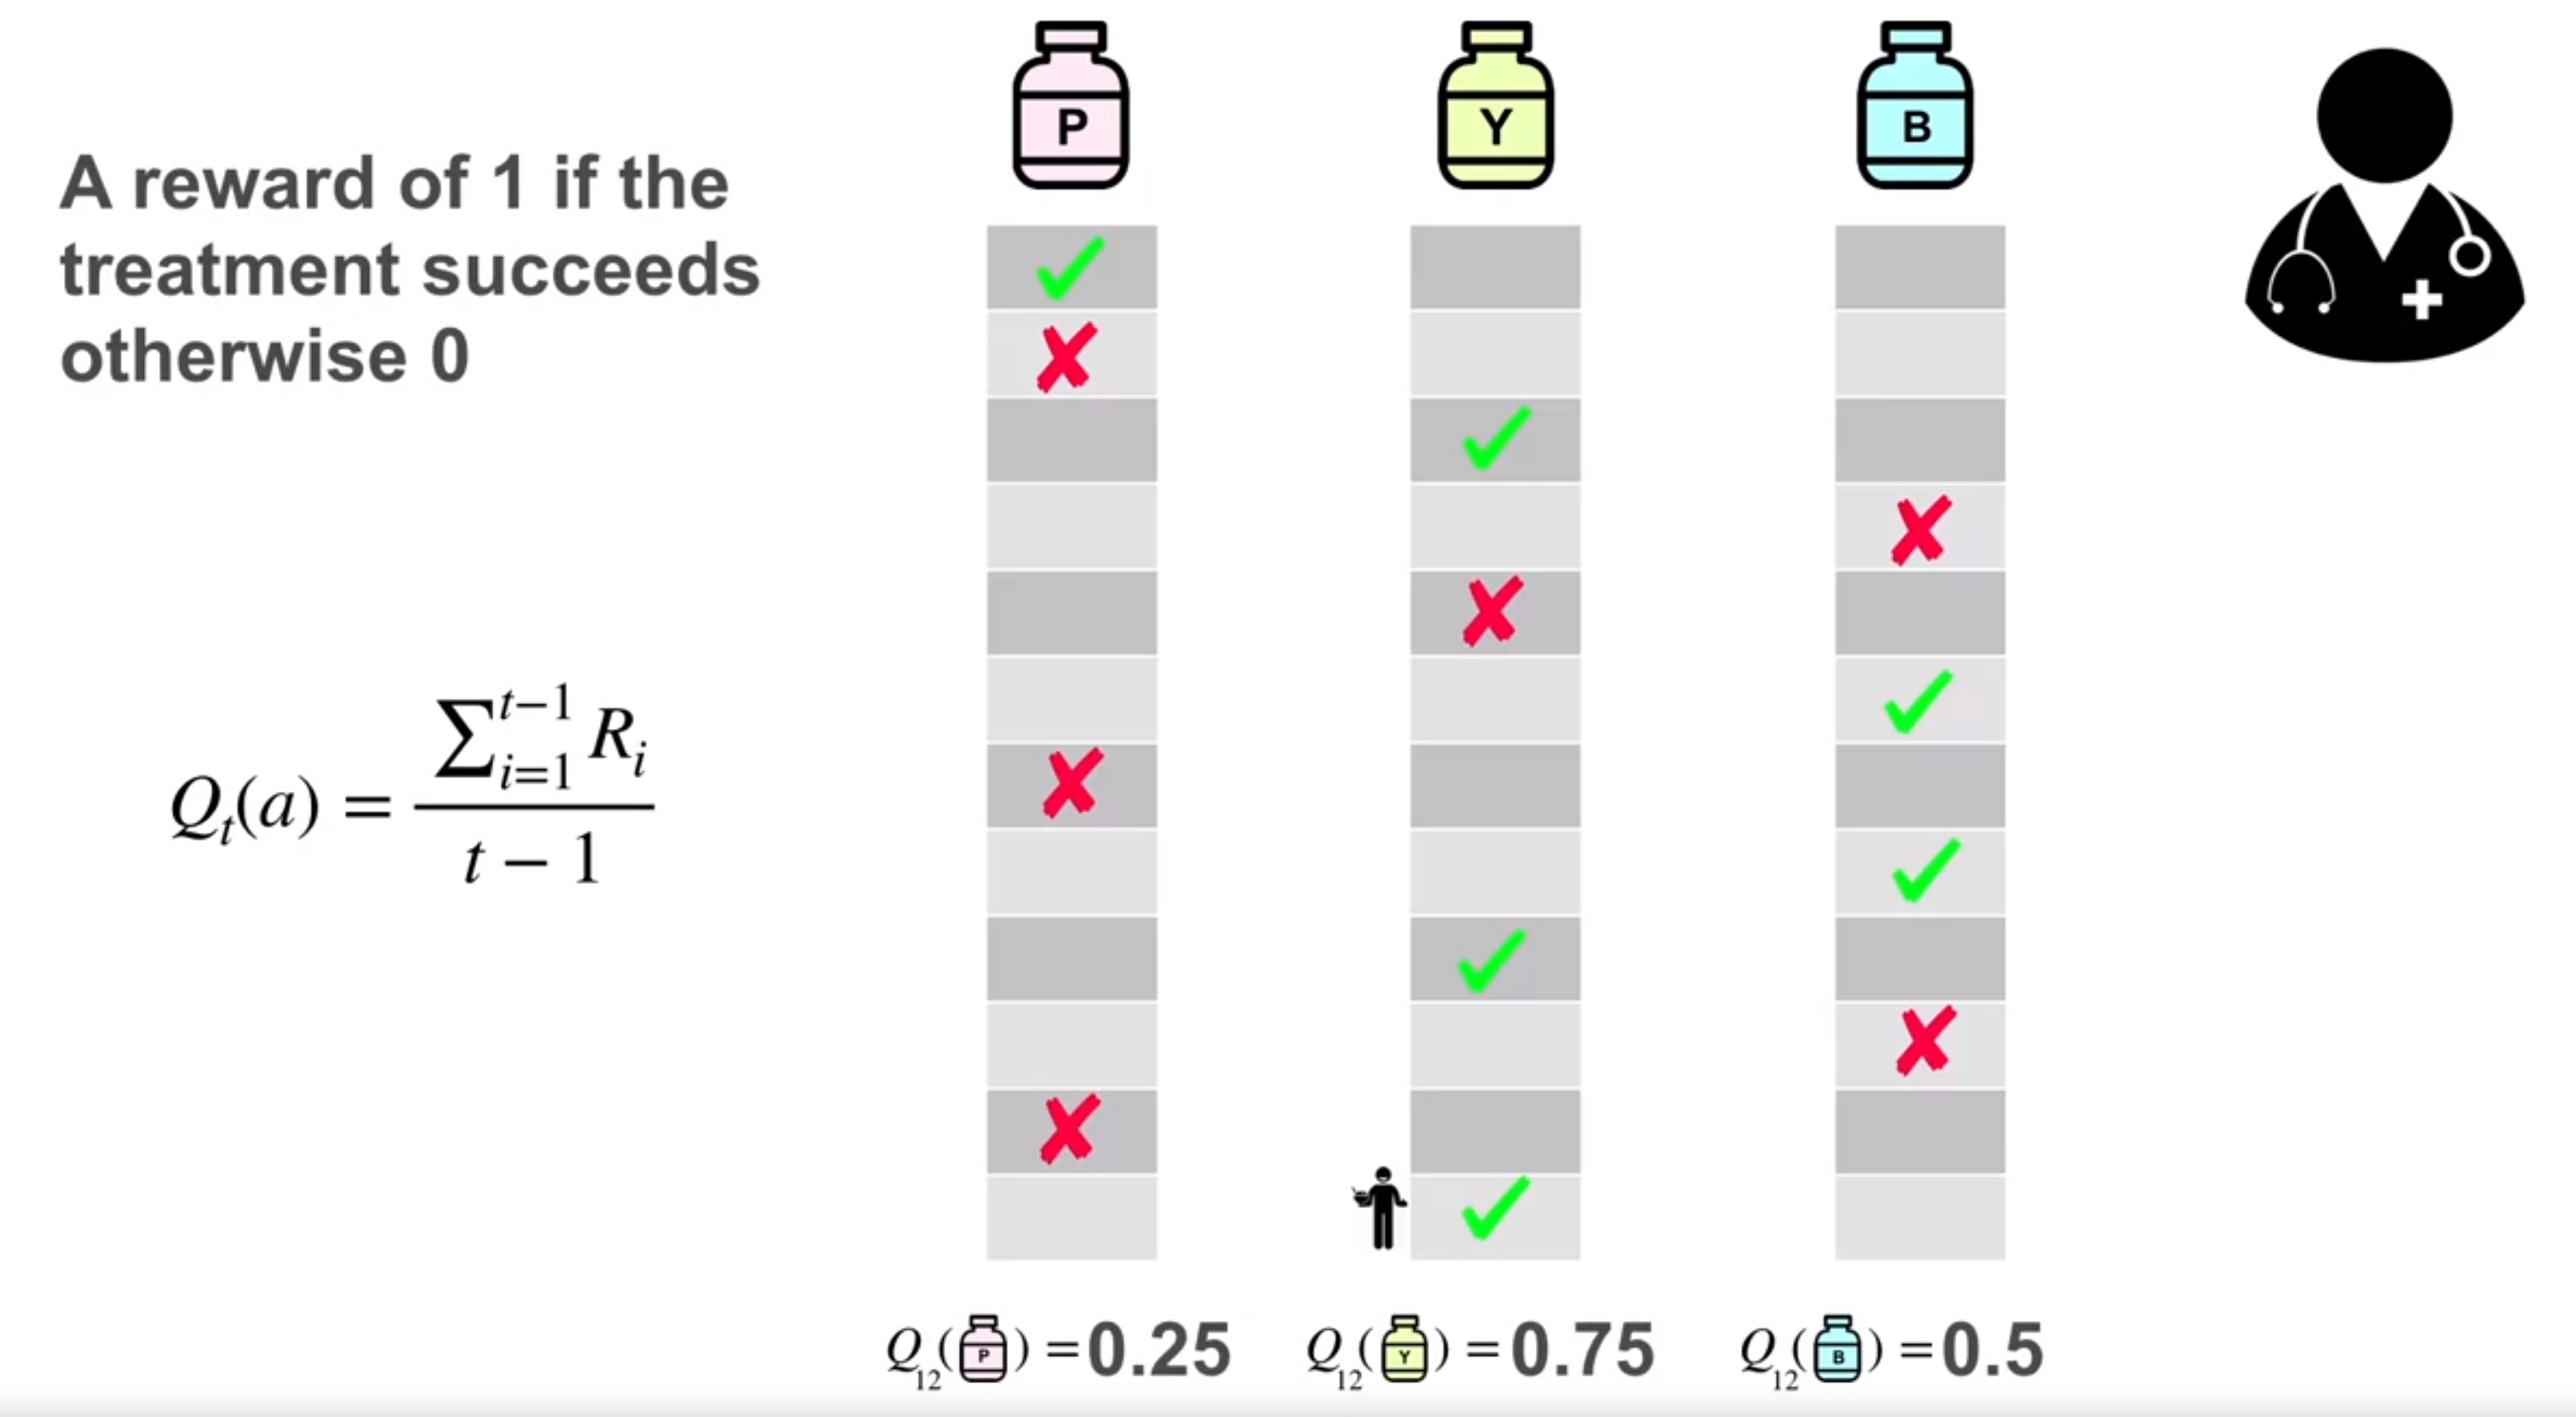
\includegraphics[keepaspectratio]{img/rl-sample-avarage-method.png}}

}

\caption{example}

\end{figure}%

\begin{equation}\phantomsection\label{eq-sample-average-incremental-update-rule}{
\begin{align}
Q_{n+1} &= \frac{1}{n} \sum_{i=1}^n R_i \newline
  & = \frac{1}{n} \Bigg(R_n + \sum_i^{n-1} R_i\Bigg) \newline
  & = \frac{1}{n} \Bigg(R_n + (n-1) \frac{1}{(n-1)}\sum_i^{n-1} R_i\Bigg) \newline
  &= \frac{1}{n} \Big(R_n + (n-1) Q_{n}\Big) \newline
  &= \frac{1}{n} \Big(R_n + nQ_{n} -Q_{n} \Big) \newline
  &= Q_n + \frac{1}{n} \Big[R_n - Q_{n}\Big]
\end{align}
}\end{equation}

\subsubsection{What are action-value estimation methods?}\label{L2G6}

We can now state this in English as:

\[
\text{New Estimate} \leftarrow \text{Old Estimate} + \text{Step Size } \times [\text{Target} - \text{Old Estimate}] \qquad
\]

here:

\begin{itemize}
\tightlist
\item
  step size can be adaptive - changing over time. but typically it is
  constant and in the range (0,1) to avoid divergence.
\item
  for the sample average method the step size is \(\frac{1}{n}\) where n
  is the number of times the action has been taken.
\item
  (Target - OldEstimate) is called the \emph{error}.
\end{itemize}

More generally we will use the update rule as:

\begin{equation}\phantomsection\label{eq-general-incremental-update-rule}{
Q_{n+1} = Q_n + \alpha \Big[R_n - Q_{n}\Big] \qquad a\in (0,1)
}\end{equation}

\begin{Shaded}
\begin{Highlighting}[]
\NormalTok{\#| label: simple{-}epsilon{-}greedy{-}bandit{-}algorithm}
\NormalTok{\#| html{-}indent{-}size: "1.2em"}
\NormalTok{\#| html{-}comment{-}delimiter: "\#"}
\NormalTok{\#| html{-}line{-}number: true}
\NormalTok{\#| html{-}line{-}number{-}punc: ":"}
\NormalTok{\#| html{-}no{-}end: false}
\NormalTok{\#| pdf{-}placement: "htb!"}
\NormalTok{\#| pdf{-}line{-}number: true}

\NormalTok{\textbackslash{}begin\{algorithm\}}
\NormalTok{\textbackslash{}caption\{Simple Bandit($\textbackslash{}epsilon$)\}}
\NormalTok{\textbackslash{}begin\{algorithmic\}[1]}
\NormalTok{\textbackslash{}State $Q(a) \textbackslash{}leftarrow 0\textbackslash{} \textbackslash{}forall a\textbackslash{} $ \textbackslash{}Comment\{ $\textbackslash{}textcolor\{blue\}\{initialize\textbackslash{} action\textbackslash{} values\}$\}}
\NormalTok{\textbackslash{}State $N(a) \textbackslash{}leftarrow 0\textbackslash{} \textbackslash{}forall a\textbackslash{} $ \textbackslash{}Comment\{ $\textbackslash{}textcolor\{blue\}\{initialize\textbackslash{} counter\textbackslash{} for\textbackslash{} actions\textbackslash{} taken\}$\}}
\NormalTok{\textbackslash{}For\{$t = 1, 2, \textbackslash{}ldots \textbackslash{}infty$\}}
\NormalTok{  \textbackslash{}State  $A\_t \textbackslash{}leftarrow \textbackslash{}begin\{cases\}}
\NormalTok{    \textbackslash{}arg\textbackslash{}max\_a Q(a) \& \textbackslash{}text\{with probability \} 1 {-} \textbackslash{}epsilon \textbackslash{}\textbackslash{}}
\NormalTok{    \textbackslash{}text\{a random action\} \& \textbackslash{}text\{with probability \} \textbackslash{}epsilon}
\NormalTok{    \textbackslash{}end\{cases\}$}
\NormalTok{  \textbackslash{}State $R\_t \textbackslash{}leftarrow \textbackslash{}text\{Bandit\}(A\_t)$}
\NormalTok{  \textbackslash{}State $N(A\_t) \textbackslash{}leftarrow N(A\_t) + 1$}
\NormalTok{  \textbackslash{}State $Q(A\_t) \textbackslash{}leftarrow Q(A\_t) + \textbackslash{}frac\{1\}\{N(A\_t)\}[R\_t {-} Q(A\_t)]$}
\NormalTok{\textbackslash{}EndFor}
\NormalTok{\textbackslash{}end\{algorithmic\}}
\NormalTok{\textbackslash{}end\{algorithm\}}
\end{Highlighting}
\end{Shaded}

\section{Lesson 3: Exploration vs
Exploitation}\label{sec-lesson-exploration-exploitation}

\begin{tcolorbox}[enhanced jigsaw, left=2mm, leftrule=.75mm, bottomtitle=1mm, toptitle=1mm, title=\textcolor{quarto-callout-note-color}{\faInfo}\hspace{0.5em}{Goals}, breakable, toprule=.15mm, colbacktitle=quarto-callout-note-color!10!white, coltitle=black, colback=white, opacityback=0, rightrule=.15mm, bottomrule=.15mm, colframe=quarto-callout-note-color-frame, titlerule=0mm, opacitybacktitle=0.6, arc=.35mm]

\begin{itemize}
\tightlist
\item
  Define \(\epsilon\)-greedy \hyperref[sec-epsilon-greedy-policies]{\#}
\item
  Compare the short-term benefits of exploitation and the long-term
  benefits of exploration
  \hyperref[sec-benefits-of-exploitation-and-exploration]{\#}
\item
  Understand optimistic initial values
  \hyperref[sec-optimistic-initial-values]{\#}
\item
  Describe the benefits of optimistic initial values for early
  exploration
  \hyperref[sec-benefits-of-optimistic-initial-values-for-early-exploration]{\#}
\item
  Explain the criticisms of optimistic initial values
  \hyperref[sec-criticisms-of-optimistic-initial-values]{\#}
\item
  Describe the upper confidence bound action selection method
  \hyperref[L3G6]{\#}
\item
  Define optimism in the face of uncertainty \hyperref[L3G7]{\#}
\end{itemize}

\end{tcolorbox}

the following is a Bernoulli greedy algorithm

\begin{Shaded}
\begin{Highlighting}[]
\NormalTok{\#| label: alg{-}greedy{-}bandit}
\NormalTok{\#| html{-}indent{-}size: "1.2em"}
\NormalTok{\#| html{-}comment{-}delimiter: "\#"}
\NormalTok{\#| html{-}line{-}number: true}
\NormalTok{\#| html{-}line{-}number{-}punc: ":"}
\NormalTok{\#| html{-}no{-}end: false}
\NormalTok{\#| pdf{-}placement: "htb!"}
\NormalTok{\#| pdf{-}line{-}number: true}

\NormalTok{\textbackslash{}begin\{algorithm\}}
\NormalTok{\textbackslash{}caption\{BernGreedy(K, α, β)\}}
\NormalTok{\textbackslash{}begin\{algorithmic\}[1]}
\NormalTok{\textbackslash{}For\{$t = 1, 2, . . .$\}}
\NormalTok{\textbackslash{}State}
\NormalTok{\textbackslash{}State \textbackslash{}Comment\{ estimate model\}}
\NormalTok{\textbackslash{}For\{$k = 1, . . . , K$\}}
\NormalTok{\textbackslash{}State $\textbackslash{}hat\textbackslash{}theta\_k \textbackslash{}leftarrow  a\_k / (α\_k + β\_k)$}
\NormalTok{\textbackslash{}EndFor}
\NormalTok{\textbackslash{}State \textbackslash{}Comment\{ select and apply action:\}}
\NormalTok{\textbackslash{}State $x\_t \textbackslash{}leftarrow \textbackslash{}arg\textbackslash{}max\_k \textbackslash{}hat\{\textbackslash{}theta\}\_k$}
\NormalTok{\textbackslash{}State Apply $x\_t$ and observe $r\_t$}
\NormalTok{\textbackslash{}State \textbackslash{}Comment\{ update distribution:\}}
\NormalTok{\textbackslash{}State $(α\_\{x\_t\}, β\_\{x\_t\}) \textbackslash{}leftarrow (α\_\{x\_t\} + r\_t, β\_\{x\_t\} + 1 − r\_t)$}
\NormalTok{\textbackslash{}EndFor}
\NormalTok{\textbackslash{}end\{algorithmic\}}
\NormalTok{\textbackslash{}end\{algorithm\}}
\end{Highlighting}
\end{Shaded}

\subsection{Ɛ-Greedy Policies}\label{sec-epsilon-greedy-policies}

The Ɛ-greedy policy uses a simple heuristic to balance exploration with
exploitation. The idea is to choose the best action with probability
\(1-\epsilon\) and to choose a random action with probability
\(\epsilon\).

\begin{Shaded}
\begin{Highlighting}[]
\NormalTok{\#| label: alg{-}epsilon{-}greedy}
\NormalTok{\#| html{-}indent{-}size: "1.2em"}
\NormalTok{\#| html{-}comment{-}delimiter: "\#"}
\NormalTok{\#| html{-}line{-}number: true}
\NormalTok{\#| html{-}line{-}number{-}punc: ":"}
\NormalTok{\#| html{-}no{-}end: false}
\NormalTok{\#| pdf{-}placement: "htb!"}
\NormalTok{\#| pdf{-}line{-}number: true}

\NormalTok{\textbackslash{}begin\{algorithm\}}
\NormalTok{\textbackslash{}caption\{EpsilonGreedy(K, α, β)\}}
\NormalTok{\textbackslash{}begin\{algorithmic\}[1]}
\NormalTok{\textbackslash{}For\{$t = 1, 2, \textbackslash{}ldots $\}}
\NormalTok{\textbackslash{}State p = random()}
\NormalTok{  \textbackslash{}If \{$p \textless{} \textbackslash{}epsilon$\}}
\NormalTok{    \textbackslash{}State select radom action $x\_t \textbackslash{}qquad$ \textbackslash{}Comment\{explore\}}
\NormalTok{  \textbackslash{}Else}
\NormalTok{    \textbackslash{}State select $x\_t = \textbackslash{}arg\textbackslash{}max\_k \textbackslash{}hat\{\textbackslash{}theta\}\_k \textbackslash{}qquad$  \textbackslash{}Comment\{exploit\}}
\NormalTok{  \textbackslash{}EndIf}
\NormalTok{\textbackslash{}EndFor}
\NormalTok{\textbackslash{}end\{algorithmic\}}
\NormalTok{\textbackslash{}end\{algorithm\}}
\end{Highlighting}
\end{Shaded}

\begin{tcolorbox}[enhanced jigsaw, left=2mm, leftrule=.75mm, bottomtitle=1mm, toptitle=1mm, title=\textcolor{quarto-callout-caution-color}{\faFire}\hspace{0.5em}{The problem with Ɛ-greedy policies}, breakable, toprule=.15mm, colbacktitle=quarto-callout-caution-color!10!white, coltitle=black, colback=white, opacityback=0, rightrule=.15mm, bottomrule=.15mm, colframe=quarto-callout-caution-color-frame, titlerule=0mm, opacitybacktitle=0.6, arc=.35mm]

\begin{itemize}
\tightlist
\item
  A problem with Ɛ-greedy is that it is not optimal in the long run.
\item
  Even after it has found the best course of action it will continue to
  explore with probability \(\epsilon\).
\item
  This is because the policy is not adaptive.
\item
  One method is too reduce \(\epsilon\) over time. However unless there
  is a feedback from the environment this will likely stop exploring too
  soon or too late thus providing sub-optimal returns.
\end{itemize}

\end{tcolorbox}

The following is a simple implementation of the Ɛ-greedy algorithm in
Python from
\href{https://www.geeksforgeeks.org/epsilon-greedy-algorithm-in-reinforcement-learning/?ref=ml_lbp}{geeksforgeeks.org}

\begin{Shaded}
\begin{Highlighting}[]
\CommentTok{\# Import required libraries }
\ImportTok{import}\NormalTok{ numpy }\ImportTok{as}\NormalTok{ np }
\ImportTok{import}\NormalTok{ matplotlib.pyplot }\ImportTok{as}\NormalTok{ plt }
  
\CommentTok{\# Define Action class }
\KeywordTok{class}\NormalTok{ Actions: }
  \KeywordTok{def} \FunctionTok{\_\_init\_\_}\NormalTok{(}\VariableTok{self}\NormalTok{, m): }
    \VariableTok{self}\NormalTok{.m }\OperatorTok{=}\NormalTok{ m }
    \VariableTok{self}\NormalTok{.mean }\OperatorTok{=} \DecValTok{0}
    \VariableTok{self}\NormalTok{.N }\OperatorTok{=} \DecValTok{0}
  
  \CommentTok{\# Choose a random action }
  \KeywordTok{def}\NormalTok{ choose(}\VariableTok{self}\NormalTok{):  }
    \ControlFlowTok{return}\NormalTok{ np.random.randn() }\OperatorTok{+} \VariableTok{self}\NormalTok{.m }
  
  \CommentTok{\# Update the action{-}value estimate }
  \KeywordTok{def}\NormalTok{ update(}\VariableTok{self}\NormalTok{, x): }
    \VariableTok{self}\NormalTok{.N }\OperatorTok{+=} \DecValTok{1}
    \VariableTok{self}\NormalTok{.mean }\OperatorTok{=}\NormalTok{ (}\DecValTok{1} \OperatorTok{{-}} \FloatTok{1.0} \OperatorTok{/} \VariableTok{self}\NormalTok{.N)}\OperatorTok{*}\VariableTok{self}\NormalTok{.mean }\OperatorTok{+} \FloatTok{1.0} \OperatorTok{/} \VariableTok{self}\NormalTok{.N }\OperatorTok{*}\NormalTok{ x }
  
  
\KeywordTok{def}\NormalTok{ run\_experiment(m1, m2, m3, eps, N): }
      
\NormalTok{  actions }\OperatorTok{=}\NormalTok{ [Actions(m1), Actions(m2), Actions(m3)] }
  
\NormalTok{  data }\OperatorTok{=}\NormalTok{ np.empty(N) }
    
  \ControlFlowTok{for}\NormalTok{ i }\KeywordTok{in} \BuiltInTok{range}\NormalTok{(N): }
    \CommentTok{\# epsilon greedy }
\NormalTok{    p }\OperatorTok{=}\NormalTok{ np.random.random() }
    \ControlFlowTok{if}\NormalTok{ p }\OperatorTok{\textless{}}\NormalTok{ eps: }
\NormalTok{      j }\OperatorTok{=}\NormalTok{ np.random.choice(}\DecValTok{3}\NormalTok{) }
    \ControlFlowTok{else}\NormalTok{: }
\NormalTok{      j }\OperatorTok{=}\NormalTok{ np.argmax([a.mean }\ControlFlowTok{for}\NormalTok{ a }\KeywordTok{in}\NormalTok{ actions]) }
\NormalTok{    x }\OperatorTok{=}\NormalTok{ actions[j].choose() }
\NormalTok{    actions[j].update(x) }
  
    \CommentTok{\# for the plot }
\NormalTok{    data[i] }\OperatorTok{=}\NormalTok{ x }
\NormalTok{  cumulative\_average }\OperatorTok{=}\NormalTok{ np.cumsum(data) }\OperatorTok{/}\NormalTok{ (np.arange(N) }\OperatorTok{+} \DecValTok{1}\NormalTok{) }
  
  \CommentTok{\# plot moving average ctr }
\NormalTok{  plt.plot(cumulative\_average) }
\NormalTok{  plt.plot(np.ones(N)}\OperatorTok{*}\NormalTok{m1) }
\NormalTok{  plt.plot(np.ones(N)}\OperatorTok{*}\NormalTok{m2) }
\NormalTok{  plt.plot(np.ones(N)}\OperatorTok{*}\NormalTok{m3) }
\NormalTok{  plt.xscale(}\StringTok{\textquotesingle{}log\textquotesingle{}}\NormalTok{) }
\NormalTok{  plt.show() }
  
  \ControlFlowTok{for}\NormalTok{ a }\KeywordTok{in}\NormalTok{ actions: }
    \BuiltInTok{print}\NormalTok{(a.mean) }
  
  \ControlFlowTok{return}\NormalTok{ cumulative\_average }
\end{Highlighting}
\end{Shaded}

\begin{Shaded}
\begin{Highlighting}[]
\NormalTok{c\_1 }\OperatorTok{=}\NormalTok{ run\_experiment(}\FloatTok{1.0}\NormalTok{, }\FloatTok{2.0}\NormalTok{, }\FloatTok{3.0}\NormalTok{, }\FloatTok{0.1}\NormalTok{, }\DecValTok{100000}\NormalTok{) }
\CommentTok{\#print(c\_1)}
\end{Highlighting}
\end{Shaded}

\pandocbounded{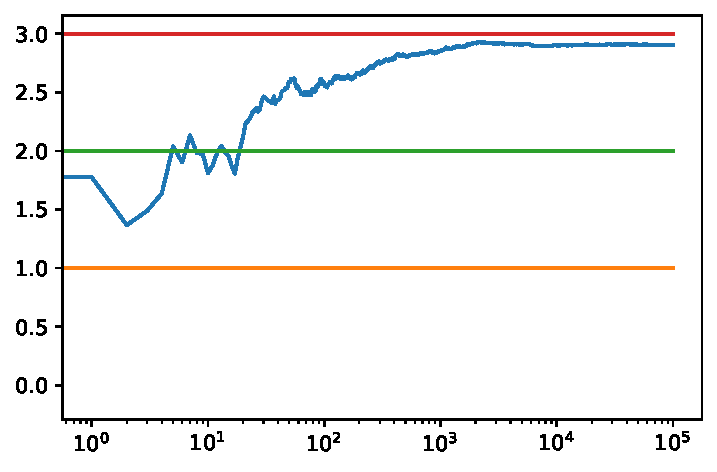
\includegraphics[keepaspectratio]{c1-w1_files/figure-pdf/cell-3-output-1.pdf}}

\begin{verbatim}
0.9731500241984946
2.005916925837013
3.002296733328393
\end{verbatim}

\begin{Shaded}
\begin{Highlighting}[]
\NormalTok{c\_05 }\OperatorTok{=}\NormalTok{ run\_experiment(}\FloatTok{1.0}\NormalTok{, }\FloatTok{2.0}\NormalTok{, }\FloatTok{3.0}\NormalTok{, }\FloatTok{0.05}\NormalTok{, }\DecValTok{100000}\NormalTok{) }
\CommentTok{\#print(c\_05)}
\end{Highlighting}
\end{Shaded}

\pandocbounded{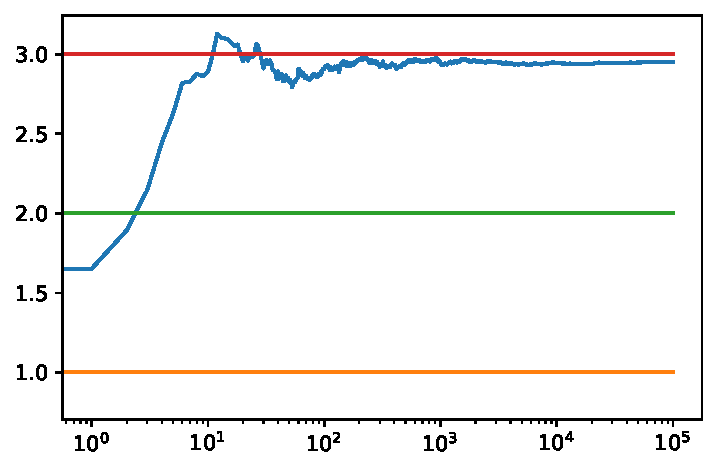
\includegraphics[keepaspectratio]{c1-w1_files/figure-pdf/cell-4-output-1.pdf}}

\begin{verbatim}
1.0315451107815639
2.0269411539772952
2.9987258631705425
\end{verbatim}

\begin{Shaded}
\begin{Highlighting}[]
\NormalTok{c\_01 }\OperatorTok{=}\NormalTok{ run\_experiment(}\FloatTok{1.0}\NormalTok{, }\FloatTok{2.0}\NormalTok{, }\FloatTok{3.0}\NormalTok{, }\FloatTok{0.01}\NormalTok{, }\DecValTok{100000}\NormalTok{) }
\CommentTok{\#print(c\_01)}
\end{Highlighting}
\end{Shaded}

\pandocbounded{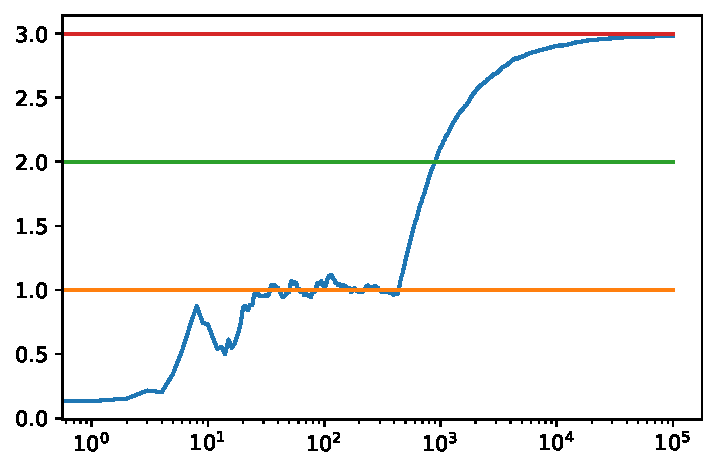
\includegraphics[keepaspectratio]{c1-w1_files/figure-pdf/cell-5-output-1.pdf}}

\begin{verbatim}
1.0074803639279672
2.026943545658896
3.001221182441492
\end{verbatim}

\begin{Shaded}
\begin{Highlighting}[]
\CommentTok{\# log scale plot }
\NormalTok{plt.plot(c\_1, label }\OperatorTok{=}\StringTok{\textquotesingle{}eps = 0.1\textquotesingle{}}\NormalTok{) }
\NormalTok{plt.plot(c\_05, label }\OperatorTok{=}\StringTok{\textquotesingle{}eps = 0.05\textquotesingle{}}\NormalTok{) }
\NormalTok{plt.plot(c\_01, label }\OperatorTok{=}\StringTok{\textquotesingle{}eps = 0.01\textquotesingle{}}\NormalTok{) }
\NormalTok{plt.legend() }
\NormalTok{plt.xscale(}\StringTok{\textquotesingle{}log\textquotesingle{}}\NormalTok{) }
\NormalTok{plt.show() }
\end{Highlighting}
\end{Shaded}

\pandocbounded{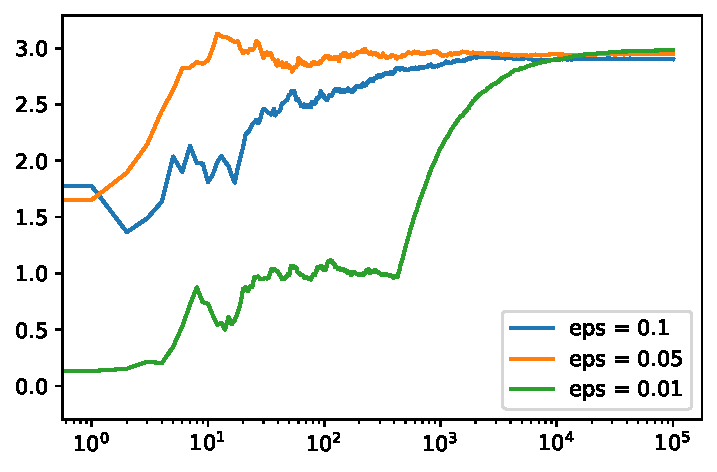
\includegraphics[keepaspectratio]{c1-w1_files/figure-pdf/cell-6-output-1.pdf}}

\subsection{Benefits of Exploitation \&
Exploration}\label{sec-benefits-of-exploitation-and-exploration}

\begin{itemize}
\tightlist
\item
  In the short term we may maximize rewards following the best known
  course of action. However this may represent a local maximum.
\item
  In the long term agents that explore different options and keep
  uncovering better options until they find the best course of action
  corresponding to the global maximum.
\end{itemize}

To get the best of both worlds we need to balance exploration and
exploitation ideally using a policy that uses feedback to adapt to its
environment.

\subsection{Optimistic initial
values}\label{sec-optimistic-initial-values}

\begin{description}
\item[Optimistic initial values]
Setting all initially action values greater than the algorithmically
available values in {[}0,1{]}
\end{description}

The methods we have discussed are dependent on the initial action-value
estimates, \(Q_1(a)\). In the language of statistics, we call these
methods biased by their initial estimates. For the sample-average
methods, the bias disappears once all actions have been selected at
least once. For methods with constant \(\alpha\), the bias is permanent,
though decreasing over time.

\begin{Shaded}
\begin{Highlighting}[]
\NormalTok{\#| label: alg{-}optimitc{-}greedy{-}bandit}
\NormalTok{\#| html{-}indent{-}size: "1.2em"}
\NormalTok{\#| html{-}comment{-}delimiter: "\#"}
\NormalTok{\#| html{-}line{-}number: true}
\NormalTok{\#| html{-}line{-}number{-}punc: ":"}
\NormalTok{\#| html{-}no{-}end: false}
\NormalTok{\#| pdf{-}placement: "htb!"}
\NormalTok{\#| pdf{-}line{-}number: true}

\NormalTok{\textbackslash{}begin\{algorithm\}}
\NormalTok{\textbackslash{}caption\{OptimisticBernGreedy(K, α, β)\}}
\NormalTok{\textbackslash{}begin\{algorithmic\}[1]}
\NormalTok{\textbackslash{}For\{$t = 1, 2, . . .$\}}
\NormalTok{\textbackslash{}State}
\NormalTok{\textbackslash{}State \textbackslash{}Comment\{ estimate model\}}
\NormalTok{\textbackslash{}For\{$k = 1, . . . , K$\}}
\NormalTok{\textbackslash{}State $\textbackslash{}hat\textbackslash{}theta\_k \textbackslash{}leftarrow  1 \textbackslash{}qquad$ \textbackslash{}Comment\{optimistic initial value\}}
\NormalTok{\textbackslash{}EndFor}
\NormalTok{\textbackslash{}State \textbackslash{}Comment\{ select and apply action:\}}
\NormalTok{\textbackslash{}State $x\_t \textbackslash{}leftarrow \textbackslash{}arg\textbackslash{}max\_k \textbackslash{}hat\{\textbackslash{}theta\}\_k$}
\NormalTok{\textbackslash{}State Apply $x\_t$ and observe $r\_t$}
\NormalTok{\textbackslash{}State \textbackslash{}Comment\{ update distribution:\}}
\NormalTok{\textbackslash{}State $(α\_\{x\_t\}, β\_\{x\_t\}) \textbackslash{}leftarrow (α\_\{x\_t\} + r\_t, β\_\{x\_t\} + 1 − r\_t)$}
\NormalTok{\textbackslash{}EndFor}
\NormalTok{\textbackslash{}end\{algorithmic\}}
\NormalTok{\textbackslash{}end\{algorithm\}}
\end{Highlighting}
\end{Shaded}

\subsection{Benefits of optimistic initial values for early
exploration}\label{sec-benefits-of-optimistic-initial-values-for-early-exploration}

Setting the initial action values to be higher than the true values has
the effect of causing various bandit algorithm to try to exploit them -
only to find out that most values are not as rewarding as it was led to
expect.

What happens is that the algorithm will initially explore more than it
would have otherwise. Possibly even trying all the actions at least
once.

In the short-term it will perform worse than Ɛ- greedy which tend to
exploit. But as more of the state space is explored at least once the
algorithm will beat an Ɛ-greedy policy which can take far longer to
explore the space and find the optimal options.

\begin{figure}[H]

{\centering \pandocbounded{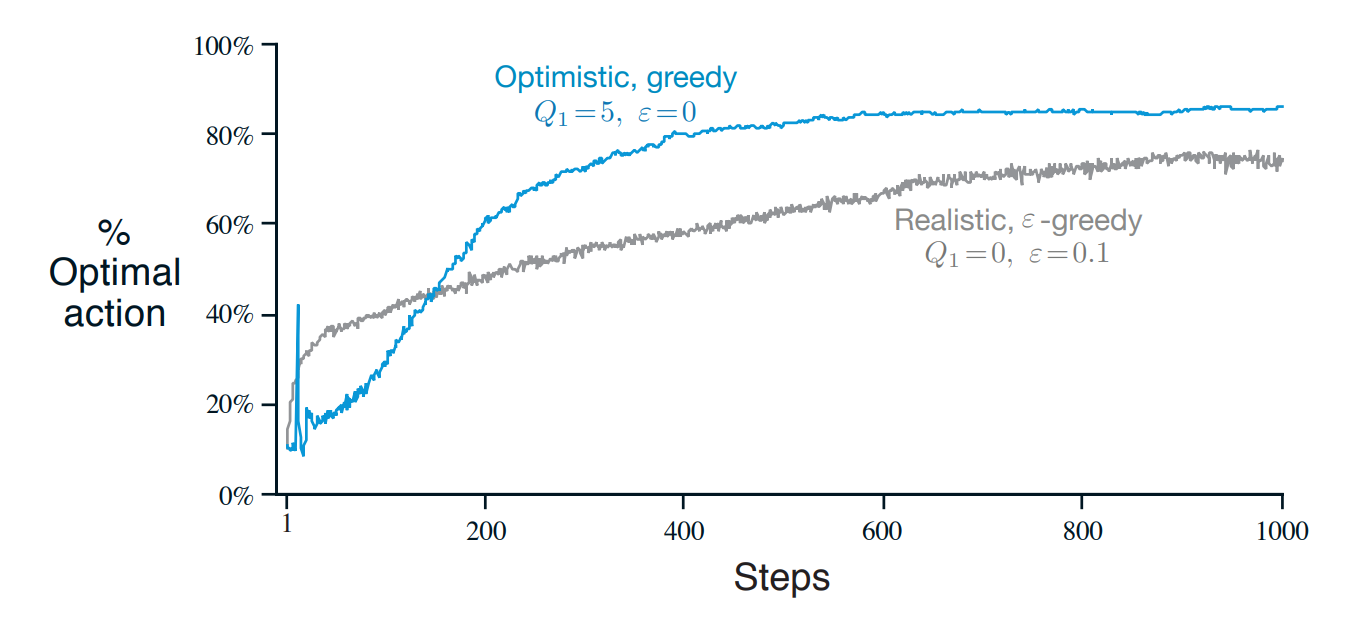
\includegraphics[keepaspectratio]{img/rl-optimistic-initial-conditions.png}}

}

\caption{The effect of optimistic initial action-value estimates}

\end{figure}%

\begin{tcolorbox}[enhanced jigsaw, left=2mm, leftrule=.75mm, bottomtitle=1mm, toptitle=1mm, title=\textcolor{quarto-callout-caution-color}{\faFire}\hspace{0.5em}{Criticisms of optimistic initial values}, breakable, toprule=.15mm, colbacktitle=quarto-callout-caution-color!10!white, coltitle=black, colback=white, opacityback=0, rightrule=.15mm, bottomrule=.15mm, colframe=quarto-callout-caution-color-frame, titlerule=0mm, opacitybacktitle=0.6, arc=.35mm]

\begin{itemize}
\tightlist
\item
  Optimistic initial values only drive early exploration. The agent will
  stop exploring once this is done.
\item
  For a non-stationary problems - this is inadequate.
\item
  In a real world problems the maximum reward is an unknown quantity.
\end{itemize}

\end{tcolorbox}

\subsection{The UCB action selection
method}\label{sec-the-ucb-action-selection-method}

UCB is an acronym for Upper Confidence Bound. The idea behind it is to
select the action that has the highest upper confidence bound. This has
the advantage over epsilon greedy that it will explore more in the
beginning and then exploit more as the algorithm progresses.

the upper confidence bound is defined as:

\begin{equation}\phantomsection\label{eq-ucb}{
A_t = \arg\max\_a \Bigg[
  \underbrace{Q_t(a)}_{exploitation} + 
  \underbrace{c \sqrt{\frac{\ln t}{N_t(a)} }}_{exploration}
\Bigg] \qquad
}\end{equation}

where:

\begin{itemize}
\tightlist
\item
  \(Q_t(a)\) is the action value
\item
  \(c\) is a constant that determines the degree of exploration
\item
  \(N_t(a)\) is the number of times action \(a\) has been selected prior
  to time \(t\)
\end{itemize}

\begin{figure}[H]

{\centering \pandocbounded{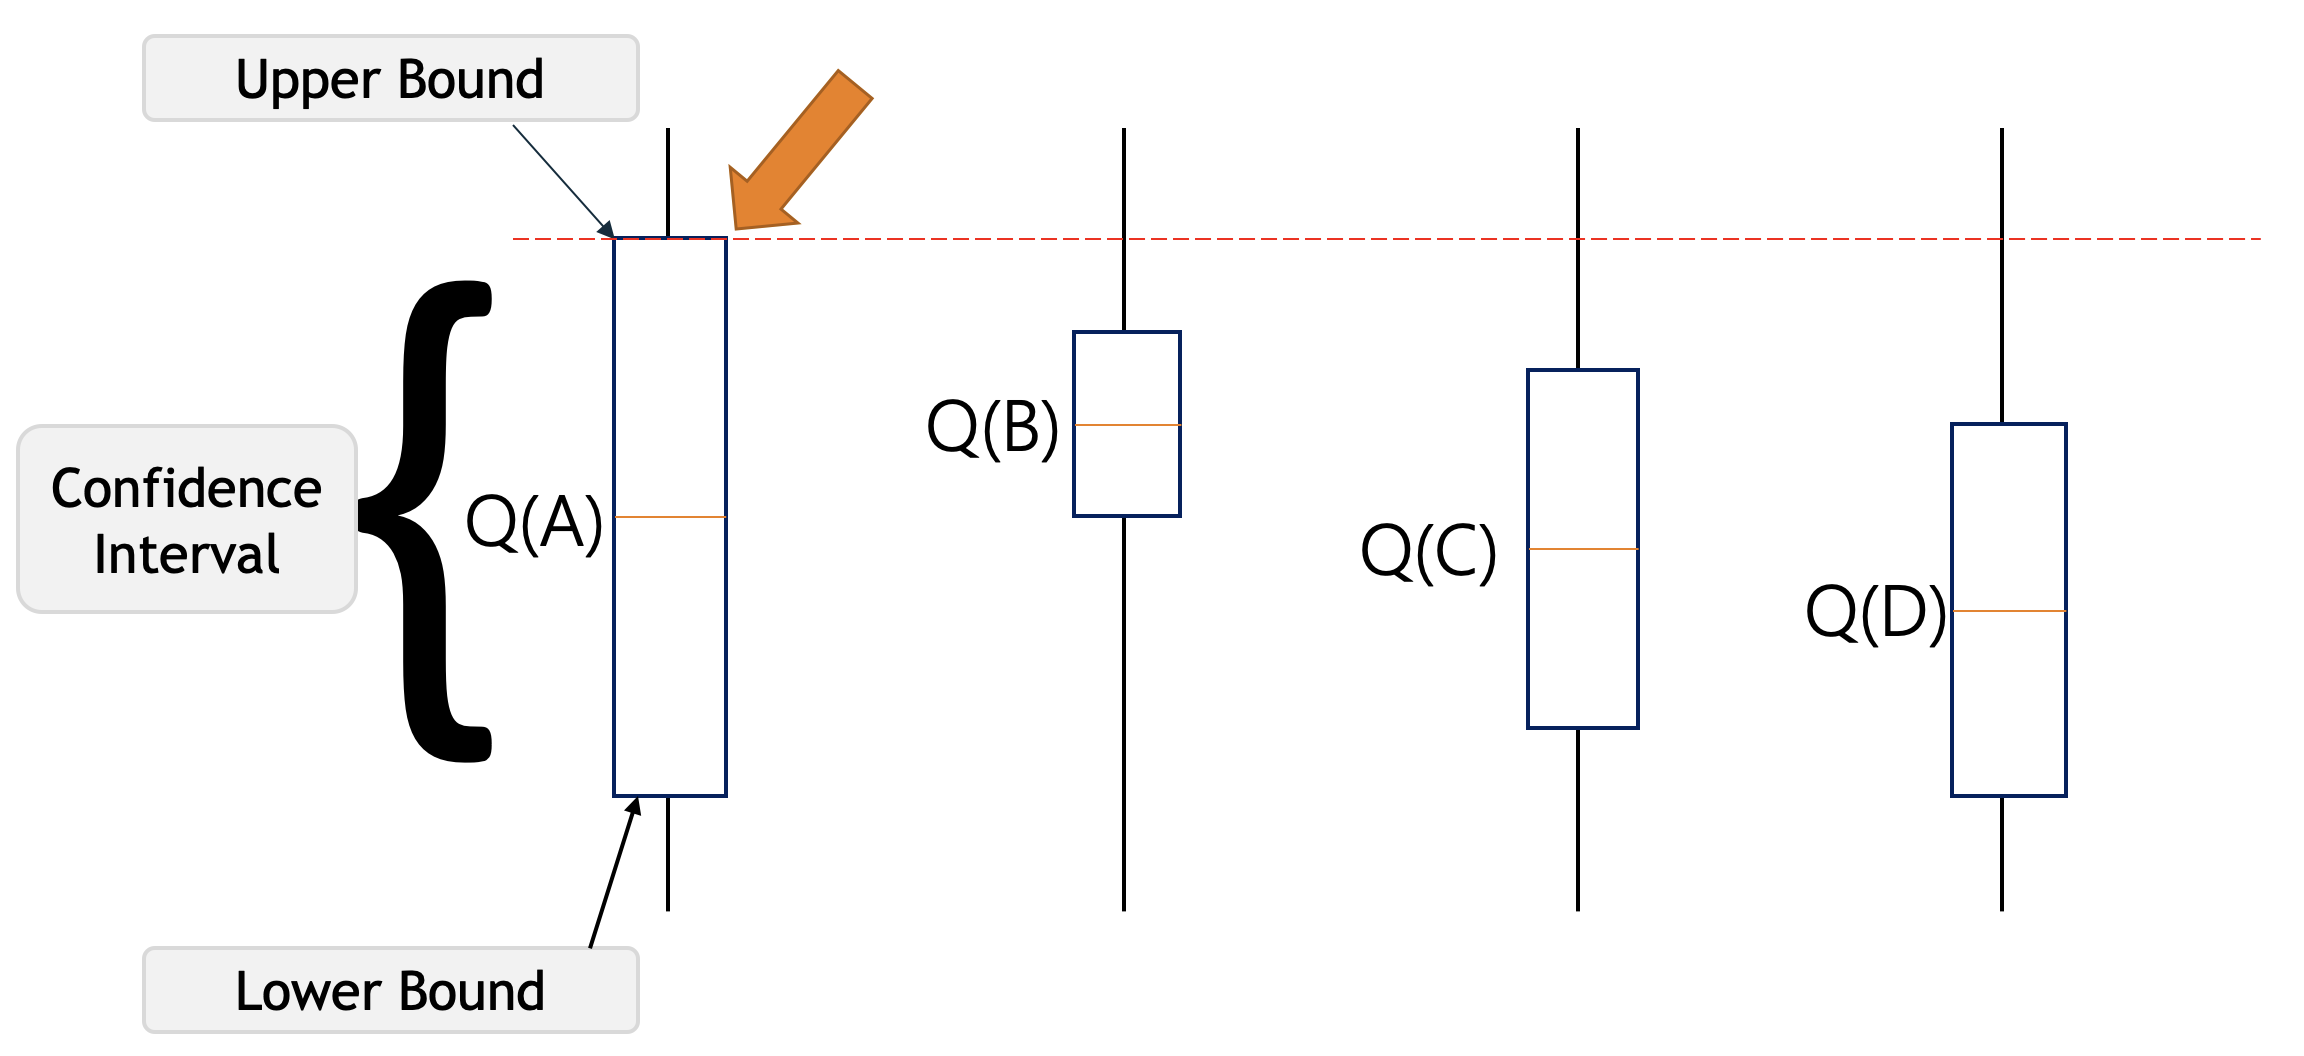
\includegraphics[keepaspectratio]{img/rl_wk1_ucb.png}}

}

\caption{UCB intuition}

\end{figure}%

The idea is we the action for which the action value plus the highest
possible uncertainty give the highest sum. We are being optimistic in
assuming this choice will give the highest reward. In reality any value
in the confidence interval could be the true value. Each time we select
an action we reduce the uncertainty in the exploration term and we also
temper our optimism of the upper confidence bound by the number of times
we have selected the action. This means that we will prefer to visit the
actions that have not been visited as often.

The main advantage of UCB is that it is more efficient than epsilon
greedy in the long run. If we measure the cost of learning in terms of
the regret - the difference between the expected reward of the optimal
action and the expected reward of the action we choose. UCB has a lower
regret than epsilon greedy. The downside is that it is more complex and
requires more computation.

\begin{Shaded}
\begin{Highlighting}[]
\NormalTok{\#| label: alg{-}brn{-}UCB}
\NormalTok{\#| html{-}indent{-}size: "1.2em"}
\NormalTok{\#| html{-}comment{-}delimiter: "\#"}
\NormalTok{\#| html{-}line{-}number: true}
\NormalTok{\#| html{-}line{-}number{-}punc: ":"}
\NormalTok{\#| html{-}no{-}end: false}
\NormalTok{\#| pdf{-}placement: "htb!"}
\NormalTok{\#| pdf{-}line{-}number: true}

\NormalTok{\textbackslash{}begin\{algorithm\}}
\NormalTok{\textbackslash{}caption\{UCB(K, α, β)\}}
\NormalTok{\textbackslash{}begin\{algorithmic\}[1]}
\NormalTok{\textbackslash{}For\{$t = 1, 2, . . .$\}}
\NormalTok{  \textbackslash{}For \{ $k = 1, . . . , K$ \}}
\NormalTok{    \textbackslash{}State \textbackslash{}Comment\{ $\textbackslash{}textcolor\{blue\}\{compute\textbackslash{} UCBs\}$\}}
\NormalTok{    \textbackslash{}State $U\_k = \textbackslash{}hat\textbackslash{}theta\_k + c \textbackslash{}sqrt\{\textbackslash{}frac\{\textbackslash{}ln t\}\{N\_k\}\}$}
\NormalTok{  \textbackslash{}EndFor}
\NormalTok{\textbackslash{}State \textbackslash{}Comment\{ $\textbackslash{}textcolor\{blue\}\{select\textbackslash{} and\textbackslash{} apply\textbackslash{} action\}$\}}
\NormalTok{\textbackslash{}State $x\_t \textbackslash{}leftarrow \textbackslash{}arg\textbackslash{}max\_k h(x,U\_x)$}
\NormalTok{\textbackslash{}State Apply xt and observe $y\_t$ and $r\_t$}
\NormalTok{\textbackslash{}State \textbackslash{}Comment\{ $\textbackslash{}textcolor\{blue\}\{estimate\textbackslash{} model\}$\}}
\NormalTok{\textbackslash{}For\{$k = 1, . . . , K$\}}
\NormalTok{\textbackslash{}State $\textbackslash{}hat\textbackslash{}theta\_k \textbackslash{}leftarrow  a\_k / (α\_k + β\_k)$}
\NormalTok{\textbackslash{}EndFor}
\NormalTok{\textbackslash{}State \textbackslash{}Comment\{ select and apply action:\}}
\NormalTok{\textbackslash{}State $x\_t \textbackslash{}leftarrow \textbackslash{}arg\textbackslash{}max\_k \textbackslash{}hat\{\textbackslash{}theta\}\_k$}
\NormalTok{\textbackslash{}State Apply $x\_t$ and observe $r\_t$}
\NormalTok{\textbackslash{}State \textbackslash{}Comment\{ update distribution:\}}
\NormalTok{\textbackslash{}State $(α\_\{x\_t\}, β\_\{x\_t\}) \textbackslash{}leftarrow (α\_\{x\_t\} + r\_t, β\_\{x\_t\} + 1 − r\_t)$}
\NormalTok{\textbackslash{}EndFor}
\NormalTok{\textbackslash{}end\{algorithmic\}}
\NormalTok{\textbackslash{}end\{algorithm\}}
\end{Highlighting}
\end{Shaded}

Note we can model UCB using an urn model.

\subsection{Thompson Sampling}\label{Sec-Thompson-Sampling}

Thompson sampling is basically like UCB but taking the Bayesian approach
to the bandit problem. We start with a prior distribution over the
action values and then update this distribution as we take actions. The
action we choose is then sampled from the posterior distribution. This
has the advantage that it is more robust to non-stationary problems than
UCB. The downside is that it is more computationally expensive.

\subsubsection{Thompson Sampling
Algorithm}\label{Sec-Thompson-Sampling-Algorithm}

The algorithm is as follows:

\begin{Shaded}
\begin{Highlighting}[]
\NormalTok{\#| label: alg{-}bernoulli{-}thompson{-}sampling}
\NormalTok{\#| html{-}indent{-}size: "1.2em"}
\NormalTok{\#| html{-}comment{-}delimiter: "\#"}
\NormalTok{\#| html{-}line{-}number: true}
\NormalTok{\#| html{-}line{-}number{-}punc: ":"}
\NormalTok{\#| html{-}no{-}end: false}
\NormalTok{\#| pdf{-}placement: "htb!"}
\NormalTok{\#| pdf{-}line{-}number: true}

\NormalTok{\textbackslash{}begin\{algorithm\}}
\NormalTok{\textbackslash{}caption\{BernTS(K, α, β)\}}
\NormalTok{\textbackslash{}begin\{algorithmic\}[1]}
\NormalTok{\textbackslash{}For\{$t = 1, 2, . . .$\}}
\NormalTok{\textbackslash{}State}
\NormalTok{\textbackslash{}State \textbackslash{}Comment\{ sample model\}}
\NormalTok{\textbackslash{}For\{$k = 1, . . . , K$\}}
\NormalTok{\textbackslash{}State Sample $\textbackslash{}hat\textbackslash{}theta\_k \textbackslash{}sim beta(α\_k, β\_k)$}
\NormalTok{\textbackslash{}EndFor}
\NormalTok{\textbackslash{}State \textbackslash{}Comment\{ select and apply action:\}}
\NormalTok{\textbackslash{}State $x\_t \textbackslash{}leftarrow \textbackslash{}arg\textbackslash{}max\_k \textbackslash{}hat\{\textbackslash{}theta\}\_k$}
\NormalTok{\textbackslash{}State Apply $x\_t$ and observe $r\_t$}
\NormalTok{\textbackslash{}State \textbackslash{}Comment\{ update distribution:\}}
\NormalTok{\textbackslash{}State $(α\_\{x\_t\}, β\_\{x\_t\}) \textbackslash{}leftarrow (α\_\{x\_t\} + r\_t, β\_\{x\_t\} + 1 − r\_t)$}
\NormalTok{\textbackslash{}EndFor}
\NormalTok{\textbackslash{}end\{algorithmic\}}
\NormalTok{\textbackslash{}end\{algorithm\}}
\end{Highlighting}
\end{Shaded}

\begin{itemize}
\tightlist
\item
  \href{https://web.stanford.edu/~bvr/pubs/TS_Tutorial.pdf}{this is a
  tutorial on Thompson Sampling}
\end{itemize}

\subsection{Optimism in the face of uncertainty}\label{L3G7}

\begin{description}
\item[Optimism in the face of uncertainty]
This is a heuristic to ensure initial exploration of all actions by
assuming that untried actions have a high expected reward. We then try
to exploit them but end up successively downgrading their expected
reward when they do not match our initial optimistic assessment.
\end{description}

The downside to this approach is when the space of action is continuous
so we can never get to the benefits of exploration.

\section{Awesome RL resources}\label{awesome-rl-resources}

Let's list some useful RL resources.

\textbf{Books}

\begin{itemize}
\tightlist
\item
  Richard S. Sutton \& Andrew G. Barto
  \href{http://incompleteideas.net/book/RLbook2020.pdf}{RL An
  Introduction}
\item
  \href{https://tor-lattimore.com/}{Tor Latimore's}
  \href{https://tor-lattimore.com/downloads/book/book.pdf}{Book} and
  \href{https://banditalgs.com/}{Blog} on Bandit Algorithms.
\item
  \href{https://sites.ualberta.ca/~szepesva/}{Csaba Szepesvari}'s
  \href{https://www.ualberta.ca/~szepesva/papers/RLAlgsInMDPs.pdf}{Book}
\end{itemize}

\textbf{Courses \& Tutorials}

\begin{itemize}
\tightlist
\item
  \href{http://www0.cs.ucl.ac.uk/staff/d.silver/web/Home.html}{David
  Silver's} 2015 \href{https://www.davidsilver.uk/teaching/}{UCL Course
  on RL} \href{https://www.youtube.com/watch?v=2pWv7GOvuf0}{Video} and
  Slides.
\item
  \href{https://faculty.cc.gatech.edu/~isbell/pubs/}{Charles Isbell} and
  \href{https://www.littmania.com/}{Michael Littman} A free Udacity
  course on RL, with some emphasis on game theory proofs, and some novel
  algorithms like
  \href{http://proceedings.mlr.press/v28/sodomka13.pdf}{Coco-Q: Learning
  in Stochastic Games with Side Payments}.
\item
  \textbf{Contextual Bandits} \href{https://hunch.net/~rwil/}{tutorial}
  \href{https://vimeo.com/240429210}{video} + papers from MS research
  videos on contextual bandit algorithms.
\item
  Interesting papers:

  \begin{itemize}
  \tightlist
  \item
    We discussed how Dynamic Programming can't handle games like chess.
    Here are some RL methods that can.

    \begin{itemize}
    \tightlist
    \item
      \href{https://www.nature.com/articles/s41586-020-03051-4.epdf?sharing_token=kTk-xTZpQOF8Ym8nTQK6EdRgN0jAjWel9jnR3ZoTv0PMSWGj38iNIyNOw_ooNp2BvzZ4nIcedo7GEXD7UmLqb0M_V_fop31mMY9VBBLNmGbm0K9jETKkZnJ9SgJ8Rwhp3ySvLuTcUr888puIYbngQ0fiMf45ZGDAQ7fUI66-u7Y\%3D}{Muzero}
    \item
      \href{https://arxiv.org/abs/2202.06626}{MuZero} and
    \item
      \href{https://arxiv.org/abs/2111.00210}{EfficentZero}
      \href{https://github.com/YeWR/EfficientZero}{code}
    \end{itemize}
  \end{itemize}
\end{itemize}

\subsection{Coding Bandits with MESA}\label{coding-bandits-with-mesa}

\begin{Shaded}
\begin{Highlighting}[]
\ImportTok{from}\NormalTok{ tqdm }\ImportTok{import}\NormalTok{ tqdm}
\ImportTok{from}\NormalTok{ mesa }\ImportTok{import}\NormalTok{ Model, Agent}
\ImportTok{from}\NormalTok{ mesa.time }\ImportTok{import}\NormalTok{ RandomActivation}
\ImportTok{import}\NormalTok{ numpy }\ImportTok{as}\NormalTok{ np}



\KeywordTok{class}\NormalTok{ EpsilonGreedyAgent(Agent):}
    \CommentTok{"""}
\CommentTok{    This agent implements the epsilon{-}greedy }
\CommentTok{    """}

    \KeywordTok{def} \FunctionTok{\_\_init\_\_}\NormalTok{(}\VariableTok{self}\NormalTok{, unique\_id, model, num\_arms, epsilon}\OperatorTok{=}\FloatTok{0.1}\NormalTok{):}
        \BuiltInTok{super}\NormalTok{().}\FunctionTok{\_\_init\_\_}\NormalTok{(unique\_id,model)}
        \VariableTok{self}\NormalTok{.num\_arms }\OperatorTok{=}\NormalTok{ num\_arms}
        \VariableTok{self}\NormalTok{.epsilon }\OperatorTok{=}\NormalTok{ epsilon}
        \VariableTok{self}\NormalTok{.q\_values }\OperatorTok{=}\NormalTok{ np.zeros(num\_arms)  }\CommentTok{\# Initialize Q{-}value estimates}
        \VariableTok{self}\NormalTok{.action\_counts }\OperatorTok{=}\NormalTok{ np.zeros(num\_arms)  }\CommentTok{\# Track action counts}

    \KeywordTok{def}\NormalTok{ choose\_action(}\VariableTok{self}\NormalTok{):}
        \ControlFlowTok{if}\NormalTok{ np.random.rand() }\OperatorTok{\textless{}} \VariableTok{self}\NormalTok{.epsilon:}
            \CommentTok{\# Exploration: Choose random arm}
            \ControlFlowTok{return}\NormalTok{ np.random.randint(}\DecValTok{0}\NormalTok{, }\VariableTok{self}\NormalTok{.num\_arms)}
        \ControlFlowTok{else}\NormalTok{:}
            \CommentTok{\# Exploitation: Choose arm with highest Q{-}value}
            \ControlFlowTok{return}\NormalTok{ np.argmax(}\VariableTok{self}\NormalTok{.q\_values)}

    \KeywordTok{def}\NormalTok{ step(}\VariableTok{self}\NormalTok{, model):}
\NormalTok{        chosen\_arm }\OperatorTok{=} \VariableTok{self}\NormalTok{.choose\_action()}
\NormalTok{        reward }\OperatorTok{=}\NormalTok{ model.get\_reward(chosen\_arm)}
        \ControlFlowTok{assert}\NormalTok{ reward }\KeywordTok{is} \KeywordTok{not} \VariableTok{None}\NormalTok{, }\StringTok{"Reward is not provided by the model"}
        \VariableTok{self}\NormalTok{.action\_counts[chosen\_arm] }\OperatorTok{+=} \DecValTok{1}
        \VariableTok{self}\NormalTok{.q\_values[chosen\_arm] }\OperatorTok{=}\NormalTok{ (}\VariableTok{self}\NormalTok{.q\_values[chosen\_arm] }\OperatorTok{*} \VariableTok{self}\NormalTok{.action\_counts[chosen\_arm] }\OperatorTok{+}\NormalTok{ reward) }\OperatorTok{/}\NormalTok{ (}\VariableTok{self}\NormalTok{.action\_counts[chosen\_arm] }\OperatorTok{+} \DecValTok{1}\NormalTok{)}


\KeywordTok{class}\NormalTok{ TestbedModel(Model):}
    \CommentTok{"""}
\CommentTok{    This model represents the 10{-}armed bandit testbed environment.}
\CommentTok{    """}

    \KeywordTok{def} \FunctionTok{\_\_init\_\_}\NormalTok{(}\VariableTok{self}\NormalTok{, num\_arms, mean\_reward, std\_dev,num\_agents}\OperatorTok{=}\DecValTok{1}\NormalTok{):}
        \BuiltInTok{super}\NormalTok{().}\FunctionTok{\_\_init\_\_}\NormalTok{()}
        \VariableTok{self}\NormalTok{.num\_agents }\OperatorTok{=}\NormalTok{ num\_agents}
        \VariableTok{self}\NormalTok{.num\_arms }\OperatorTok{=}\NormalTok{ num\_arms}
        \VariableTok{self}\NormalTok{.mean\_reward }\OperatorTok{=}\NormalTok{ mean\_reward}
        \VariableTok{self}\NormalTok{.std\_dev }\OperatorTok{=}\NormalTok{ std\_dev}
        \VariableTok{self}\NormalTok{.env\_init()}
        \CommentTok{\#self.arms = [None] * num\_arms  \# List to store arm rewards}
        \VariableTok{self}\NormalTok{.schedule }\OperatorTok{=}\NormalTok{ RandomActivation(}\VariableTok{self}\NormalTok{)}
        \ControlFlowTok{for}\NormalTok{ i }\KeywordTok{in} \BuiltInTok{range}\NormalTok{(}\VariableTok{self}\NormalTok{.num\_agents):}
          \VariableTok{self}\NormalTok{.create\_agent(EpsilonGreedyAgent, i, }\FloatTok{0.1}\NormalTok{) }

    \KeywordTok{def}\NormalTok{ env\_init(}\VariableTok{self}\NormalTok{,env\_info}\OperatorTok{=}\NormalTok{\{\}):}
        \VariableTok{self}\NormalTok{.arms }\OperatorTok{=}\NormalTok{ np.random.randn(}\VariableTok{self}\NormalTok{.num\_arms)  }\CommentTok{\# Initialize arm rewards}

    \KeywordTok{def}\NormalTok{ create\_agent(}\VariableTok{self}\NormalTok{, agent\_class, agent\_id, epsilon):}
        \CommentTok{"""}
\CommentTok{        Create an RL agent instance with the specified class and parameters.}
\CommentTok{        """}
\NormalTok{        agent }\OperatorTok{=}\NormalTok{ agent\_class(agent\_id, }\VariableTok{self}\NormalTok{, }\VariableTok{self}\NormalTok{.num\_arms, epsilon)}
        \VariableTok{self}\NormalTok{.schedule.add(agent)}
        \ControlFlowTok{return}\NormalTok{ agent}

    \KeywordTok{def}\NormalTok{ step(}\VariableTok{self}\NormalTok{):}
        \ControlFlowTok{for}\NormalTok{ agent }\KeywordTok{in} \VariableTok{self}\NormalTok{.schedule.agents:}
\NormalTok{            chosen\_arm }\OperatorTok{=}\NormalTok{ agent.choose\_action()}
\NormalTok{            reward }\OperatorTok{=}\NormalTok{ np.random.normal(}\VariableTok{self}\NormalTok{.mean\_reward, }\VariableTok{self}\NormalTok{.std\_dev)}
            \VariableTok{self}\NormalTok{.arms[chosen\_arm] }\OperatorTok{=}\NormalTok{ reward  }\CommentTok{\# Update arm reward in the model}
\NormalTok{            agent.step(}\VariableTok{self}\NormalTok{)  }\CommentTok{\# Pass the model instance to the agent for reward access}

    \KeywordTok{def}\NormalTok{ get\_reward(}\VariableTok{self}\NormalTok{, arm\_id):}
        \CommentTok{\# Access reward from the stored list}
        \ControlFlowTok{return} \VariableTok{self}\NormalTok{.arms[arm\_id]}


\CommentTok{\# Example usage}
\NormalTok{model }\OperatorTok{=}\NormalTok{ TestbedModel(}\DecValTok{10}\NormalTok{, }\DecValTok{0}\NormalTok{, }\DecValTok{1}\NormalTok{)  }\CommentTok{\# Create model with 10 arms}
\NormalTok{num\_runs }\OperatorTok{=} \DecValTok{200}                  \CommentTok{\# The number of times we run the experiment}
\NormalTok{num\_steps }\OperatorTok{=} \DecValTok{1000}                \CommentTok{\# The number of pulls of each arm the agent takes}


\CommentTok{\# Run simulation for multiple steps}
\ControlFlowTok{for}\NormalTok{ \_ }\KeywordTok{in}\NormalTok{ tqdm(}\BuiltInTok{range}\NormalTok{(num\_runs)):}
    \ControlFlowTok{for}\NormalTok{ \_ }\KeywordTok{in} \BuiltInTok{range}\NormalTok{(num\_steps):}
\NormalTok{        model.step()}
\NormalTok{    model.step()}
\end{Highlighting}
\end{Shaded}

\begin{verbatim}
  0%|          | 0/200 [00:00<?, ?it/s]  4%|▍         | 9/200 [00:00<00:02, 84.88it/s]  9%|▉         | 18/200 [00:00<00:02, 79.51it/s] 13%|█▎        | 26/200 [00:00<00:02, 78.75it/s] 17%|█▋        | 34/200 [00:00<00:02, 77.54it/s] 21%|██        | 42/200 [00:00<00:02, 75.16it/s] 25%|██▌       | 50/200 [00:00<00:01, 75.86it/s] 29%|██▉       | 58/200 [00:00<00:01, 75.36it/s] 33%|███▎      | 66/200 [00:00<00:01, 76.13it/s] 37%|███▋      | 74/200 [00:00<00:01, 76.49it/s] 41%|████      | 82/200 [00:01<00:01, 76.89it/s] 46%|████▌     | 91/200 [00:01<00:01, 78.10it/s] 50%|████▉     | 99/200 [00:01<00:01, 78.54it/s] 54%|█████▎    | 107/200 [00:01<00:01, 78.46it/s] 57%|█████▊    | 115/200 [00:01<00:01, 78.31it/s] 62%|██████▏   | 123/200 [00:01<00:00, 78.25it/s] 66%|██████▌   | 132/200 [00:01<00:00, 78.91it/s] 70%|███████   | 140/200 [00:01<00:00, 78.78it/s] 74%|███████▍  | 148/200 [00:01<00:00, 78.51it/s] 78%|███████▊  | 157/200 [00:02<00:00, 79.16it/s] 82%|████████▎ | 165/200 [00:02<00:00, 78.79it/s] 86%|████████▋ | 173/200 [00:02<00:00, 78.72it/s] 90%|█████████ | 181/200 [00:02<00:00, 78.46it/s] 94%|█████████▍| 189/200 [00:02<00:00, 78.09it/s] 98%|█████████▊| 197/200 [00:02<00:00, 78.56it/s]100%|██████████| 200/200 [00:02<00:00, 78.02it/s]
\end{verbatim}




\end{document}
